\documentclass[twoside]{book}

% Packages required by doxygen
\usepackage{fixltx2e}
\usepackage{calc}
\usepackage{doxygen}
\usepackage[export]{adjustbox} % also loads graphicx
\usepackage{graphicx}
\usepackage[utf8]{inputenc}
\usepackage{makeidx}
\usepackage{multicol}
\usepackage{multirow}
\PassOptionsToPackage{warn}{textcomp}
\usepackage{textcomp}
\usepackage[nointegrals]{wasysym}
\usepackage[table]{xcolor}

% Font selection
\usepackage[T1]{fontenc}
\usepackage[scaled=.90]{helvet}
\usepackage{courier}
\usepackage{amssymb}
\usepackage{sectsty}
\renewcommand{\familydefault}{\sfdefault}
\allsectionsfont{%
  \fontseries{bc}\selectfont%
  \color{darkgray}%
}
\renewcommand{\DoxyLabelFont}{%
  \fontseries{bc}\selectfont%
  \color{darkgray}%
}
\newcommand{\+}{\discretionary{\mbox{\scriptsize$\hookleftarrow$}}{}{}}

% Page & text layout
\usepackage{geometry}
\geometry{%
  a4paper,%
  top=2.5cm,%
  bottom=2.5cm,%
  left=2.5cm,%
  right=2.5cm%
}
\tolerance=750
\hfuzz=15pt
\hbadness=750
\setlength{\emergencystretch}{15pt}
\setlength{\parindent}{0cm}
\setlength{\parskip}{3ex plus 2ex minus 2ex}
\makeatletter
\renewcommand{\paragraph}{%
  \@startsection{paragraph}{4}{0ex}{-1.0ex}{1.0ex}{%
    \normalfont\normalsize\bfseries\SS@parafont%
  }%
}
\renewcommand{\subparagraph}{%
  \@startsection{subparagraph}{5}{0ex}{-1.0ex}{1.0ex}{%
    \normalfont\normalsize\bfseries\SS@subparafont%
  }%
}
\makeatother

% Headers & footers
\usepackage{fancyhdr}
\pagestyle{fancyplain}
\fancyhead[LE]{\fancyplain{}{\bfseries\thepage}}
\fancyhead[CE]{\fancyplain{}{}}
\fancyhead[RE]{\fancyplain{}{\bfseries\leftmark}}
\fancyhead[LO]{\fancyplain{}{\bfseries\rightmark}}
\fancyhead[CO]{\fancyplain{}{}}
\fancyhead[RO]{\fancyplain{}{\bfseries\thepage}}
\fancyfoot[LE]{\fancyplain{}{}}
\fancyfoot[CE]{\fancyplain{}{}}
\fancyfoot[RE]{\fancyplain{}{\bfseries\scriptsize Generated by Doxygen }}
\fancyfoot[LO]{\fancyplain{}{\bfseries\scriptsize Generated by Doxygen }}
\fancyfoot[CO]{\fancyplain{}{}}
\fancyfoot[RO]{\fancyplain{}{}}
\renewcommand{\footrulewidth}{0.4pt}
\renewcommand{\chaptermark}[1]{%
  \markboth{#1}{}%
}
\renewcommand{\sectionmark}[1]{%
  \markright{\thesection\ #1}%
}

% Indices & bibliography
\usepackage{natbib}
\usepackage[titles]{tocloft}
\setcounter{tocdepth}{3}
\setcounter{secnumdepth}{5}
\makeindex

% Hyperlinks (required, but should be loaded last)
\usepackage{ifpdf}
\ifpdf
  \usepackage[pdftex,pagebackref=true]{hyperref}
\else
  \usepackage[ps2pdf,pagebackref=true]{hyperref}
\fi
\hypersetup{%
  colorlinks=true,%
  linkcolor=blue,%
  citecolor=blue,%
  unicode%
}

% Custom commands
\newcommand{\clearemptydoublepage}{%
  \newpage{\pagestyle{empty}\cleardoublepage}%
}

\usepackage{caption}
\captionsetup{labelsep=space,justification=centering,font={bf},singlelinecheck=off,skip=4pt,position=top}

%===== C O N T E N T S =====

\begin{document}

% Titlepage & ToC
\hypersetup{pageanchor=false,
             bookmarksnumbered=true,
             pdfencoding=unicode
            }
\pagenumbering{alph}
\begin{titlepage}
\vspace*{7cm}
\begin{center}%
{\Large tp3\+\_\+ex3-\/3 }\\
\vspace*{1cm}
{\large Generated by Doxygen 1.8.13}\\
\end{center}
\end{titlepage}
\clearemptydoublepage
\pagenumbering{roman}
\tableofcontents
\clearemptydoublepage
\pagenumbering{arabic}
\hypersetup{pageanchor=true}

%--- Begin generated contents ---
\chapter{Data Structure Index}
\section{Data Structures}
Here are the data structures with brief descriptions\+:\begin{DoxyCompactList}
\item\contentsline{section}{\hyperlink{struct__json__array}{\+\_\+json\+\_\+array} }{\pageref{struct__json__array}}{}
\item\contentsline{section}{\hyperlink{struct__json__object}{\+\_\+json\+\_\+object} }{\pageref{struct__json__object}}{}
\item\contentsline{section}{\hyperlink{struct__json__pair}{\+\_\+json\+\_\+pair} }{\pageref{struct__json__pair}}{}
\item\contentsline{section}{\hyperlink{struct__json__value__container}{\+\_\+json\+\_\+value\+\_\+container} }{\pageref{struct__json__value__container}}{}
\item\contentsline{section}{\hyperlink{structJsonArray}{Json\+Array} \\*Pour les tableau \char`\"{}array\char`\"{} }{\pageref{structJsonArray}}{}
\item\contentsline{section}{\hyperlink{structJsonObject}{Json\+Object} \\*Pour stoker un objet J\+S\+ON }{\pageref{structJsonObject}}{}
\item\contentsline{section}{\hyperlink{structJsonPair}{Json\+Pair} \\*Pour stocker une \char`\"{}pair\char`\"{} string \+: value }{\pageref{structJsonPair}}{}
\item\contentsline{section}{\hyperlink{unionJsonValue}{Json\+Value} \\*Pour stocker \char`\"{}value\char`\"{} }{\pageref{unionJsonValue}}{}
\item\contentsline{section}{\hyperlink{structJsonValueContainer}{Json\+Value\+Container} \\*Pour stocker \char`\"{}value\char`\"{} et son type }{\pageref{structJsonValueContainer}}{}
\item\contentsline{section}{\hyperlink{structTIntPile}{T\+Int\+Pile} \\*Structure contenant une pile d\textquotesingle{}entiers }{\pageref{structTIntPile}}{}
\item\contentsline{section}{\hyperlink{structTLex}{T\+Lex} \\*Structure contenant tous les parametres/donnees pour l\textquotesingle{}analyse lexicale }{\pageref{structTLex}}{}
\item\contentsline{section}{\hyperlink{structTSymbole}{T\+Symbole} \\*Union permettant de manipuler un entier/reel/chaine pour la table des symboles }{\pageref{structTSymbole}}{}
\item\contentsline{section}{\hyperlink{structTVoidPile}{T\+Void\+Pile} \\*Structure contenant une pile de pointeur void $\ast$ }{\pageref{structTVoidPile}}{}
\end{DoxyCompactList}

\chapter{File Index}
\section{File List}
Here is a list of all documented files with brief descriptions\+:\begin{DoxyCompactList}
\item\contentsline{section}{include/\hyperlink{json__tree_8h}{json\+\_\+tree.\+h} \\*Implemente la mise en memoire d\textquotesingle{}un arbre json }{\pageref{json__tree_8h}}{}
\item\contentsline{section}{include/\hyperlink{pile_8h}{pile.\+h} \\*Gestion d\textquotesingle{}une pile }{\pageref{pile_8h}}{}
\item\contentsline{section}{include/\hyperlink{tp2__lex_8h}{tp2\+\_\+lex.\+h} \\*Analyseur lexical pour le langage J\+S\+ON }{\pageref{tp2__lex_8h}}{}
\item\contentsline{section}{include/{\bfseries tp3\+\_\+a.\+h} }{\pageref{tp3__a_8h}}{}
\item\contentsline{section}{src/\hyperlink{json__tree_8c}{json\+\_\+tree.\+c} \\*Implemente la mise en memoire d\textquotesingle{}un arbre json }{\pageref{json__tree_8c}}{}
\item\contentsline{section}{src/\hyperlink{pile_8c}{pile.\+c} \\*Gestion d\textquotesingle{}une pile }{\pageref{pile_8c}}{}
\item\contentsline{section}{src/\hyperlink{tp2__lex_8c}{tp2\+\_\+lex.\+c} \\*Analyseur lexical pour le langage J\+S\+ON }{\pageref{tp2__lex_8c}}{}
\end{DoxyCompactList}

\chapter{Data Structure Documentation}
\hypertarget{struct__json__array}{}\section{\+\_\+json\+\_\+array Struct Reference}
\label{struct__json__array}\index{\+\_\+json\+\_\+array@{\+\_\+json\+\_\+array}}


Collaboration diagram for \+\_\+json\+\_\+array\+:\nopagebreak
\begin{figure}[H]
\begin{center}
\leavevmode
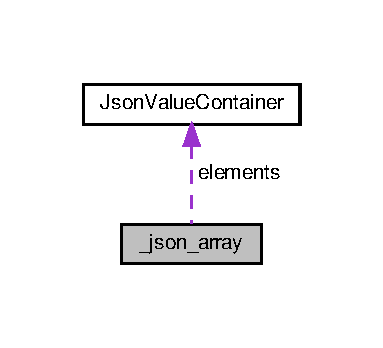
\includegraphics[width=184pt]{struct__json__array__coll__graph}
\end{center}
\end{figure}
\subsection*{Data Fields}
\begin{DoxyCompactItemize}
\item 
\hyperlink{structJsonValueContainer}{Json\+Value\+Container} $\ast$$\ast$ \hyperlink{struct__json__array_a8ca54d1e67425573f05976a454a07fd5}{elements}
\item 
int \hyperlink{struct__json__array_a94e78470cab37adc7200c745981e917f}{size}
\end{DoxyCompactItemize}


\subsection{Field Documentation}
\mbox{\Hypertarget{struct__json__array_a8ca54d1e67425573f05976a454a07fd5}\label{struct__json__array_a8ca54d1e67425573f05976a454a07fd5}} 
\index{\+\_\+json\+\_\+array@{\+\_\+json\+\_\+array}!elements@{elements}}
\index{elements@{elements}!\+\_\+json\+\_\+array@{\+\_\+json\+\_\+array}}
\subsubsection{\texorpdfstring{elements}{elements}}
{\footnotesize\ttfamily \hyperlink{structJsonValueContainer}{Json\+Value\+Container}$\ast$$\ast$ \+\_\+json\+\_\+array\+::elements}

liste des elements \mbox{\Hypertarget{struct__json__array_a94e78470cab37adc7200c745981e917f}\label{struct__json__array_a94e78470cab37adc7200c745981e917f}} 
\index{\+\_\+json\+\_\+array@{\+\_\+json\+\_\+array}!size@{size}}
\index{size@{size}!\+\_\+json\+\_\+array@{\+\_\+json\+\_\+array}}
\subsubsection{\texorpdfstring{size}{size}}
{\footnotesize\ttfamily int \+\_\+json\+\_\+array\+::size}

nombre d\textquotesingle{}elements 

The documentation for this struct was generated from the following file\+:\begin{DoxyCompactItemize}
\item 
include/\hyperlink{json__tree_8h}{json\+\_\+tree.\+h}\end{DoxyCompactItemize}

\hypertarget{struct__json__object}{}\section{\+\_\+json\+\_\+object Struct Reference}
\label{struct__json__object}\index{\+\_\+json\+\_\+object@{\+\_\+json\+\_\+object}}


Collaboration diagram for \+\_\+json\+\_\+object\+:\nopagebreak
\begin{figure}[H]
\begin{center}
\leavevmode
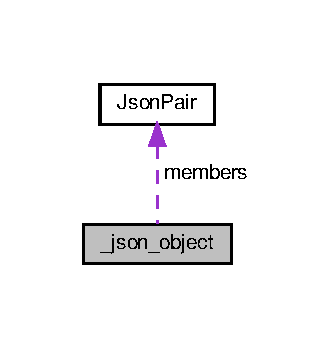
\includegraphics[width=160pt]{struct__json__object__coll__graph}
\end{center}
\end{figure}
\subsection*{Data Fields}
\begin{DoxyCompactItemize}
\item 
\hyperlink{structJsonPair}{Json\+Pair} $\ast$$\ast$ \hyperlink{struct__json__object_a61878c36cde83d313c094bb7b2a246f0}{members}
\item 
int \hyperlink{struct__json__object_a9a4c68b8224ec222391597f4e27ea447}{size}
\end{DoxyCompactItemize}


\subsection{Field Documentation}
\mbox{\Hypertarget{struct__json__object_a61878c36cde83d313c094bb7b2a246f0}\label{struct__json__object_a61878c36cde83d313c094bb7b2a246f0}} 
\index{\+\_\+json\+\_\+object@{\+\_\+json\+\_\+object}!members@{members}}
\index{members@{members}!\+\_\+json\+\_\+object@{\+\_\+json\+\_\+object}}
\subsubsection{\texorpdfstring{members}{members}}
{\footnotesize\ttfamily \hyperlink{structJsonPair}{Json\+Pair}$\ast$$\ast$ \+\_\+json\+\_\+object\+::members}

liste des membres \mbox{\Hypertarget{struct__json__object_a9a4c68b8224ec222391597f4e27ea447}\label{struct__json__object_a9a4c68b8224ec222391597f4e27ea447}} 
\index{\+\_\+json\+\_\+object@{\+\_\+json\+\_\+object}!size@{size}}
\index{size@{size}!\+\_\+json\+\_\+object@{\+\_\+json\+\_\+object}}
\subsubsection{\texorpdfstring{size}{size}}
{\footnotesize\ttfamily int \+\_\+json\+\_\+object\+::size}

nombre de membre 

The documentation for this struct was generated from the following file\+:\begin{DoxyCompactItemize}
\item 
include/\hyperlink{json__tree_8h}{json\+\_\+tree.\+h}\end{DoxyCompactItemize}

\hypertarget{struct__json__pair}{}\section{\+\_\+json\+\_\+pair Struct Reference}
\label{struct__json__pair}\index{\+\_\+json\+\_\+pair@{\+\_\+json\+\_\+pair}}


Collaboration diagram for \+\_\+json\+\_\+pair\+:\nopagebreak
\begin{figure}[H]
\begin{center}
\leavevmode
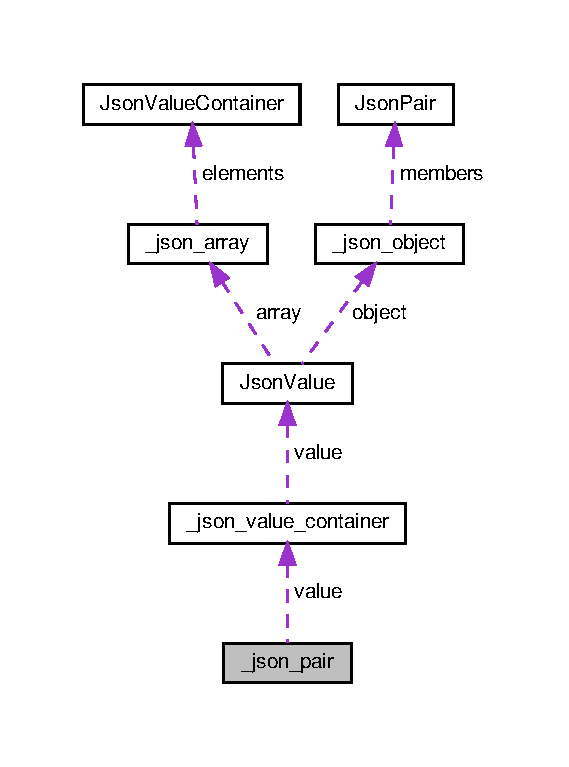
\includegraphics[width=273pt]{struct__json__pair__coll__graph}
\end{center}
\end{figure}
\subsection*{Data Fields}
\begin{DoxyCompactItemize}
\item 
char $\ast$ \hyperlink{struct__json__pair_ad599f0ce62f57e7465046444953b6275}{string}
\item 
struct \hyperlink{struct__json__value__container}{\+\_\+json\+\_\+value\+\_\+container} $\ast$ \hyperlink{struct__json__pair_a70e763b09977d01bdc56afc59fd44989}{value}
\end{DoxyCompactItemize}


\subsection{Field Documentation}
\mbox{\Hypertarget{struct__json__pair_ad599f0ce62f57e7465046444953b6275}\label{struct__json__pair_ad599f0ce62f57e7465046444953b6275}} 
\index{\+\_\+json\+\_\+pair@{\+\_\+json\+\_\+pair}!string@{string}}
\index{string@{string}!\+\_\+json\+\_\+pair@{\+\_\+json\+\_\+pair}}
\subsubsection{\texorpdfstring{string}{string}}
{\footnotesize\ttfamily char$\ast$ \+\_\+json\+\_\+pair\+::string}

name \mbox{\Hypertarget{struct__json__pair_a70e763b09977d01bdc56afc59fd44989}\label{struct__json__pair_a70e763b09977d01bdc56afc59fd44989}} 
\index{\+\_\+json\+\_\+pair@{\+\_\+json\+\_\+pair}!value@{value}}
\index{value@{value}!\+\_\+json\+\_\+pair@{\+\_\+json\+\_\+pair}}
\subsubsection{\texorpdfstring{value}{value}}
{\footnotesize\ttfamily struct \hyperlink{struct__json__value__container}{\+\_\+json\+\_\+value\+\_\+container}$\ast$ \+\_\+json\+\_\+pair\+::value}

value 

The documentation for this struct was generated from the following file\+:\begin{DoxyCompactItemize}
\item 
include/\hyperlink{json__tree_8h}{json\+\_\+tree.\+h}\end{DoxyCompactItemize}

\hypertarget{struct__json__value__container}{}\section{\+\_\+json\+\_\+value\+\_\+container Struct Reference}
\label{struct__json__value__container}\index{\+\_\+json\+\_\+value\+\_\+container@{\+\_\+json\+\_\+value\+\_\+container}}


Collaboration diagram for \+\_\+json\+\_\+value\+\_\+container\+:\nopagebreak
\begin{figure}[H]
\begin{center}
\leavevmode
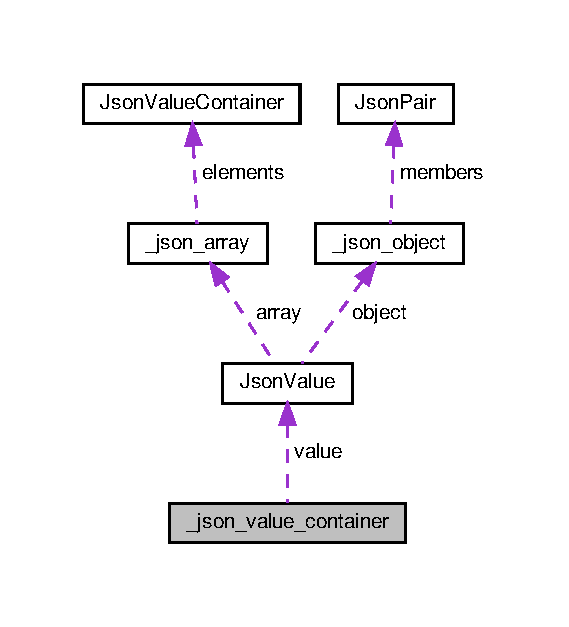
\includegraphics[width=273pt]{struct__json__value__container__coll__graph}
\end{center}
\end{figure}
\subsection*{Data Fields}
\begin{DoxyCompactItemize}
\item 
Value\+Type \hyperlink{struct__json__value__container_a21cdc2a7c5df1f10e0b61ee6f99c3bcc}{type}
\item 
\mbox{\Hypertarget{struct__json__value__container_a73ad9502b6b086e7429f69817bc7ba4b}\label{struct__json__value__container_a73ad9502b6b086e7429f69817bc7ba4b}} 
\hyperlink{unionJsonValue}{Json\+Value} {\bfseries value}
\end{DoxyCompactItemize}


\subsection{Field Documentation}
\mbox{\Hypertarget{struct__json__value__container_a21cdc2a7c5df1f10e0b61ee6f99c3bcc}\label{struct__json__value__container_a21cdc2a7c5df1f10e0b61ee6f99c3bcc}} 
\index{\+\_\+json\+\_\+value\+\_\+container@{\+\_\+json\+\_\+value\+\_\+container}!type@{type}}
\index{type@{type}!\+\_\+json\+\_\+value\+\_\+container@{\+\_\+json\+\_\+value\+\_\+container}}
\subsubsection{\texorpdfstring{type}{type}}
{\footnotesize\ttfamily Value\+Type \+\_\+json\+\_\+value\+\_\+container\+::type}

type de valeur 

The documentation for this struct was generated from the following file\+:\begin{DoxyCompactItemize}
\item 
include/\hyperlink{json__tree_8h}{json\+\_\+tree.\+h}\end{DoxyCompactItemize}

\hypertarget{structJsonArray}{}\section{Json\+Array Struct Reference}
\label{structJsonArray}\index{Json\+Array@{Json\+Array}}


pour les tableau \char`\"{}array\char`\"{}  




{\ttfamily \#include $<$json\+\_\+tree.\+h$>$}



\subsection{Detailed Description}
pour les tableau \char`\"{}array\char`\"{} 

The documentation for this struct was generated from the following file\+:\begin{DoxyCompactItemize}
\item 
include/\hyperlink{json__tree_8h}{json\+\_\+tree.\+h}\end{DoxyCompactItemize}

\hypertarget{structJsonObject}{}\section{Json\+Object Struct Reference}
\label{structJsonObject}\index{Json\+Object@{Json\+Object}}


pour stoker un objet J\+S\+ON  




{\ttfamily \#include $<$json\+\_\+tree.\+h$>$}



\subsection{Detailed Description}
pour stoker un objet J\+S\+ON 

The documentation for this struct was generated from the following file\+:\begin{DoxyCompactItemize}
\item 
include/\hyperlink{json__tree_8h}{json\+\_\+tree.\+h}\end{DoxyCompactItemize}

\hypertarget{structJsonPair}{}\section{Json\+Pair Struct Reference}
\label{structJsonPair}\index{Json\+Pair@{Json\+Pair}}


pour stocker une \char`\"{}pair\char`\"{} string \+: value  




{\ttfamily \#include $<$json\+\_\+tree.\+h$>$}



\subsection{Detailed Description}
pour stocker une \char`\"{}pair\char`\"{} string \+: value 

The documentation for this struct was generated from the following file\+:\begin{DoxyCompactItemize}
\item 
include/\hyperlink{json__tree_8h}{json\+\_\+tree.\+h}\end{DoxyCompactItemize}

\hypertarget{unionJsonValue}{}\section{Json\+Value Union Reference}
\label{unionJsonValue}\index{Json\+Value@{Json\+Value}}


pour stocker \char`\"{}value\char`\"{}  




{\ttfamily \#include $<$json\+\_\+tree.\+h$>$}



Collaboration diagram for Json\+Value\+:\nopagebreak
\begin{figure}[H]
\begin{center}
\leavevmode
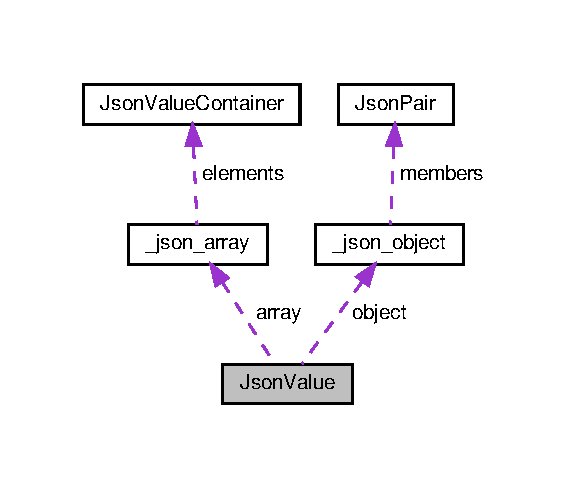
\includegraphics[width=273pt]{unionJsonValue__coll__graph}
\end{center}
\end{figure}
\subsection*{Data Fields}
\begin{DoxyCompactItemize}
\item 
\mbox{\Hypertarget{unionJsonValue_abfc034211c14bf442394b50cd9bd25c3}\label{unionJsonValue_abfc034211c14bf442394b50cd9bd25c3}} 
char $\ast$ {\bfseries string}
\item 
\mbox{\Hypertarget{unionJsonValue_a8ad081bed26b75c17d904fe0259190ce}\label{unionJsonValue_a8ad081bed26b75c17d904fe0259190ce}} 
int {\bfseries integer}
\item 
\mbox{\Hypertarget{unionJsonValue_a7ab518d4c29bdc56ea65e72ba984872d}\label{unionJsonValue_a7ab518d4c29bdc56ea65e72ba984872d}} 
float {\bfseries real}
\item 
\mbox{\Hypertarget{unionJsonValue_a634382a792f07e862035cb971746c34d}\label{unionJsonValue_a634382a792f07e862035cb971746c34d}} 
struct \hyperlink{struct__json__object}{\+\_\+json\+\_\+object} $\ast$ {\bfseries object}
\item 
\mbox{\Hypertarget{unionJsonValue_a29a36d35245a375e447f14ee321d0011}\label{unionJsonValue_a29a36d35245a375e447f14ee321d0011}} 
struct \hyperlink{struct__json__array}{\+\_\+json\+\_\+array} $\ast$ {\bfseries array}
\item 
\mbox{\Hypertarget{unionJsonValue_a3c63422483d2ea2c4c3bff331c274cbe}\label{unionJsonValue_a3c63422483d2ea2c4c3bff331c274cbe}} 
int {\bfseries constant}
\end{DoxyCompactItemize}


\subsection{Detailed Description}
pour stocker \char`\"{}value\char`\"{} 

The documentation for this union was generated from the following file\+:\begin{DoxyCompactItemize}
\item 
include/\hyperlink{json__tree_8h}{json\+\_\+tree.\+h}\end{DoxyCompactItemize}

\hypertarget{structJsonValueContainer}{}\section{Json\+Value\+Container Struct Reference}
\label{structJsonValueContainer}\index{Json\+Value\+Container@{Json\+Value\+Container}}


pour stocker \char`\"{}value\char`\"{} et son type  




{\ttfamily \#include $<$json\+\_\+tree.\+h$>$}



\subsection{Detailed Description}
pour stocker \char`\"{}value\char`\"{} et son type 

The documentation for this struct was generated from the following file\+:\begin{DoxyCompactItemize}
\item 
include/\hyperlink{json__tree_8h}{json\+\_\+tree.\+h}\end{DoxyCompactItemize}

\hypertarget{structTIntPile}{}\section{T\+Int\+Pile Struct Reference}
\label{structTIntPile}\index{T\+Int\+Pile@{T\+Int\+Pile}}


structure contenant une pile d\textquotesingle{}entiers  




{\ttfamily \#include $<$pile.\+h$>$}

\subsection*{Data Fields}
\begin{DoxyCompactItemize}
\item 
int $\ast$ \hyperlink{structTIntPile_a35035a280ee323ce10d5b5186cf85885}{data}
\item 
int \hyperlink{structTIntPile_abc42e6db26a0f0a8faec95c5f0326a1f}{index\+Sommet}
\item 
int \hyperlink{structTIntPile_a69b5112feaa16a029b4a86ec1130dec2}{size}
\end{DoxyCompactItemize}


\subsection{Detailed Description}
structure contenant une pile d\textquotesingle{}entiers 

pile contenant des entiers 

\subsection{Field Documentation}
\mbox{\Hypertarget{structTIntPile_a35035a280ee323ce10d5b5186cf85885}\label{structTIntPile_a35035a280ee323ce10d5b5186cf85885}} 
\index{T\+Int\+Pile@{T\+Int\+Pile}!data@{data}}
\index{data@{data}!T\+Int\+Pile@{T\+Int\+Pile}}
\subsubsection{\texorpdfstring{data}{data}}
{\footnotesize\ttfamily int$\ast$ T\+Int\+Pile\+::data}

tableau d\textquotesingle{}entiers representant la pile \mbox{\Hypertarget{structTIntPile_abc42e6db26a0f0a8faec95c5f0326a1f}\label{structTIntPile_abc42e6db26a0f0a8faec95c5f0326a1f}} 
\index{T\+Int\+Pile@{T\+Int\+Pile}!index\+Sommet@{index\+Sommet}}
\index{index\+Sommet@{index\+Sommet}!T\+Int\+Pile@{T\+Int\+Pile}}
\subsubsection{\texorpdfstring{index\+Sommet}{indexSommet}}
{\footnotesize\ttfamily int T\+Int\+Pile\+::index\+Sommet}

indice du sommet \mbox{\Hypertarget{structTIntPile_a69b5112feaa16a029b4a86ec1130dec2}\label{structTIntPile_a69b5112feaa16a029b4a86ec1130dec2}} 
\index{T\+Int\+Pile@{T\+Int\+Pile}!size@{size}}
\index{size@{size}!T\+Int\+Pile@{T\+Int\+Pile}}
\subsubsection{\texorpdfstring{size}{size}}
{\footnotesize\ttfamily int T\+Int\+Pile\+::size}

taille en mémoire de la pile 

The documentation for this struct was generated from the following file\+:\begin{DoxyCompactItemize}
\item 
include/\hyperlink{pile_8h}{pile.\+h}\end{DoxyCompactItemize}

\hypertarget{structTLex}{}\section{T\+Lex Struct Reference}
\label{structTLex}\index{T\+Lex@{T\+Lex}}


structure contenant tous les parametres/donnees pour l\textquotesingle{}analyse lexicale  




{\ttfamily \#include $<$tp2\+\_\+lex.\+h$>$}



Collaboration diagram for T\+Lex\+:\nopagebreak
\begin{figure}[H]
\begin{center}
\leavevmode
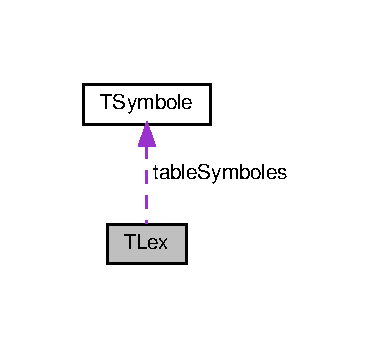
\includegraphics[width=179pt]{structTLex__coll__graph}
\end{center}
\end{figure}
\subsection*{Data Fields}
\begin{DoxyCompactItemize}
\item 
char $\ast$ \hyperlink{structTLex_a2242e630c3f871659c3e36b101b504b4}{data}
\item 
char $\ast$ \hyperlink{structTLex_a1122e1ced17c2c07f7975b4f11110ad8}{start\+Pos}
\item 
int \hyperlink{structTLex_a74499b75b25dc1bce1fb2f66af6ce1e2}{nb\+Lignes}
\item 
\hyperlink{structTSymbole}{T\+Symbole} $\ast$ \hyperlink{structTLex_a31a6c4fc0839643e3251a372ba7adf04}{table\+Symboles}
\item 
int \hyperlink{structTLex_a84d0d3a30f4b42f8db675f8cbb60373f}{nb\+Symboles}
\item 
int \hyperlink{structTLex_abb50eca8f47fc2c73983a5909967e362}{taille\+Table\+Symboles}
\end{DoxyCompactItemize}


\subsection{Detailed Description}
structure contenant tous les parametres/donnees pour l\textquotesingle{}analyse lexicale 

\subsection{Field Documentation}
\mbox{\Hypertarget{structTLex_a2242e630c3f871659c3e36b101b504b4}\label{structTLex_a2242e630c3f871659c3e36b101b504b4}} 
\index{T\+Lex@{T\+Lex}!data@{data}}
\index{data@{data}!T\+Lex@{T\+Lex}}
\subsubsection{\texorpdfstring{data}{data}}
{\footnotesize\ttfamily char$\ast$ T\+Lex\+::data}

chaine a parcourir \mbox{\Hypertarget{structTLex_a74499b75b25dc1bce1fb2f66af6ce1e2}\label{structTLex_a74499b75b25dc1bce1fb2f66af6ce1e2}} 
\index{T\+Lex@{T\+Lex}!nb\+Lignes@{nb\+Lignes}}
\index{nb\+Lignes@{nb\+Lignes}!T\+Lex@{T\+Lex}}
\subsubsection{\texorpdfstring{nb\+Lignes}{nbLignes}}
{\footnotesize\ttfamily int T\+Lex\+::nb\+Lignes}

nb de lignes analysees \mbox{\Hypertarget{structTLex_a84d0d3a30f4b42f8db675f8cbb60373f}\label{structTLex_a84d0d3a30f4b42f8db675f8cbb60373f}} 
\index{T\+Lex@{T\+Lex}!nb\+Symboles@{nb\+Symboles}}
\index{nb\+Symboles@{nb\+Symboles}!T\+Lex@{T\+Lex}}
\subsubsection{\texorpdfstring{nb\+Symboles}{nbSymboles}}
{\footnotesize\ttfamily int T\+Lex\+::nb\+Symboles}

nb de symboles stockes dans table\+Symboles \mbox{\Hypertarget{structTLex_a1122e1ced17c2c07f7975b4f11110ad8}\label{structTLex_a1122e1ced17c2c07f7975b4f11110ad8}} 
\index{T\+Lex@{T\+Lex}!start\+Pos@{start\+Pos}}
\index{start\+Pos@{start\+Pos}!T\+Lex@{T\+Lex}}
\subsubsection{\texorpdfstring{start\+Pos}{startPos}}
{\footnotesize\ttfamily char$\ast$ T\+Lex\+::start\+Pos}

position de depart pour la prochaine analyse \mbox{\Hypertarget{structTLex_a31a6c4fc0839643e3251a372ba7adf04}\label{structTLex_a31a6c4fc0839643e3251a372ba7adf04}} 
\index{T\+Lex@{T\+Lex}!table\+Symboles@{table\+Symboles}}
\index{table\+Symboles@{table\+Symboles}!T\+Lex@{T\+Lex}}
\subsubsection{\texorpdfstring{table\+Symboles}{tableSymboles}}
{\footnotesize\ttfamily \hyperlink{structTSymbole}{T\+Symbole}$\ast$ T\+Lex\+::table\+Symboles}

tableau des symboles \+: chaines/entier/reel \mbox{\Hypertarget{structTLex_abb50eca8f47fc2c73983a5909967e362}\label{structTLex_abb50eca8f47fc2c73983a5909967e362}} 
\index{T\+Lex@{T\+Lex}!taille\+Table\+Symboles@{taille\+Table\+Symboles}}
\index{taille\+Table\+Symboles@{taille\+Table\+Symboles}!T\+Lex@{T\+Lex}}
\subsubsection{\texorpdfstring{taille\+Table\+Symboles}{tailleTableSymboles}}
{\footnotesize\ttfamily int T\+Lex\+::taille\+Table\+Symboles}

taille memoire du tableau table\+Symboles 

The documentation for this struct was generated from the following file\+:\begin{DoxyCompactItemize}
\item 
include/\hyperlink{tp2__lex_8h}{tp2\+\_\+lex.\+h}\end{DoxyCompactItemize}

\hypertarget{structTSymbole}{}\section{T\+Symbole Union Reference}
\label{structTSymbole}\index{T\+Symbole@{T\+Symbole}}


union permettant de manipuler un entier/reel/chaine pour la table des symboles  




{\ttfamily \#include $<$tp2\+\_\+lex.\+h$>$}

\subsection*{Data Fields}
\begin{DoxyCompactItemize}
\item 
int \hyperlink{structTSymbole_a3f1c09d456d42f56c7e97b767fcda611}{type}
\item 
\begin{tabbing}
xx\=xx\=xx\=xx\=xx\=xx\=xx\=xx\=xx\=\kill
union \{\\
\>int {\bfseries entier}\\
\>float {\bfseries reel}\\
\>char $\ast$ {\bfseries chaine}\\
\} \hyperlink{structTSymbole_a448dc40c2c8e5d050436fa598f528723}{val}\\

\end{tabbing}\end{DoxyCompactItemize}


\subsection{Detailed Description}
union permettant de manipuler un entier/reel/chaine pour la table des symboles 

\subsection{Field Documentation}
\mbox{\Hypertarget{structTSymbole_a3f1c09d456d42f56c7e97b767fcda611}\label{structTSymbole_a3f1c09d456d42f56c7e97b767fcda611}} 
\index{T\+Symbole@{T\+Symbole}!type@{type}}
\index{type@{type}!T\+Symbole@{T\+Symbole}}
\subsubsection{\texorpdfstring{type}{type}}
{\footnotesize\ttfamily int T\+Symbole\+::type}

l\textquotesingle{}un des 3 types suivants \+: J\+S\+O\+N\+\_\+\+S\+T\+R\+I\+N\+G/\+J\+S\+O\+N\+\_\+\+I\+N\+T\+\_\+\+N\+U\+M\+B\+E\+R/ J\+S\+O\+N\+\_\+\+R\+E\+A\+L\+\_\+\+N\+U\+M\+B\+ER \mbox{\Hypertarget{structTSymbole_a448dc40c2c8e5d050436fa598f528723}\label{structTSymbole_a448dc40c2c8e5d050436fa598f528723}} 
\index{T\+Symbole@{T\+Symbole}!val@{val}}
\index{val@{val}!T\+Symbole@{T\+Symbole}}
\subsubsection{\texorpdfstring{val}{val}}
{\footnotesize\ttfamily union \{ ... \}   T\+Symbole\+::val}

valeur associer a un element de la table des symboles 

The documentation for this union was generated from the following file\+:\begin{DoxyCompactItemize}
\item 
include/\hyperlink{tp2__lex_8h}{tp2\+\_\+lex.\+h}\end{DoxyCompactItemize}

\hypertarget{structTVoidPile}{}\section{T\+Void\+Pile Struct Reference}
\label{structTVoidPile}\index{T\+Void\+Pile@{T\+Void\+Pile}}


structure contenant une pile de pointeur void $\ast$  




{\ttfamily \#include $<$pile.\+h$>$}

\subsection*{Data Fields}
\begin{DoxyCompactItemize}
\item 
void $\ast$$\ast$ \hyperlink{structTVoidPile_acca3cd1682326b767142e204d1b5d0eb}{data}
\item 
int \hyperlink{structTVoidPile_a4ec92ed494b0e73198d9dbc81818fb91}{index\+Sommet}
\item 
int \hyperlink{structTVoidPile_a1c5535f494a3c080f0ee15e615105895}{size}
\end{DoxyCompactItemize}


\subsection{Detailed Description}
structure contenant une pile de pointeur void $\ast$ 

pile contenant des pointeurs sur des objets 

\subsection{Field Documentation}
\mbox{\Hypertarget{structTVoidPile_acca3cd1682326b767142e204d1b5d0eb}\label{structTVoidPile_acca3cd1682326b767142e204d1b5d0eb}} 
\index{T\+Void\+Pile@{T\+Void\+Pile}!data@{data}}
\index{data@{data}!T\+Void\+Pile@{T\+Void\+Pile}}
\subsubsection{\texorpdfstring{data}{data}}
{\footnotesize\ttfamily void$\ast$$\ast$ T\+Void\+Pile\+::data}

tableau de pointeur void $\ast$ \mbox{\Hypertarget{structTVoidPile_a4ec92ed494b0e73198d9dbc81818fb91}\label{structTVoidPile_a4ec92ed494b0e73198d9dbc81818fb91}} 
\index{T\+Void\+Pile@{T\+Void\+Pile}!index\+Sommet@{index\+Sommet}}
\index{index\+Sommet@{index\+Sommet}!T\+Void\+Pile@{T\+Void\+Pile}}
\subsubsection{\texorpdfstring{index\+Sommet}{indexSommet}}
{\footnotesize\ttfamily int T\+Void\+Pile\+::index\+Sommet}

indice du sommet \mbox{\Hypertarget{structTVoidPile_a1c5535f494a3c080f0ee15e615105895}\label{structTVoidPile_a1c5535f494a3c080f0ee15e615105895}} 
\index{T\+Void\+Pile@{T\+Void\+Pile}!size@{size}}
\index{size@{size}!T\+Void\+Pile@{T\+Void\+Pile}}
\subsubsection{\texorpdfstring{size}{size}}
{\footnotesize\ttfamily int T\+Void\+Pile\+::size}

taille en memoire de la pile 

The documentation for this struct was generated from the following file\+:\begin{DoxyCompactItemize}
\item 
include/\hyperlink{pile_8h}{pile.\+h}\end{DoxyCompactItemize}

\chapter{File Documentation}
\hypertarget{json__tree_8h}{}\section{include/json\+\_\+tree.h File Reference}
\label{json__tree_8h}\index{include/json\+\_\+tree.\+h@{include/json\+\_\+tree.\+h}}


implemente la mise en memoire d\textquotesingle{}un arbre json  


This graph shows which files directly or indirectly include this file\+:\nopagebreak
\begin{figure}[H]
\begin{center}
\leavevmode
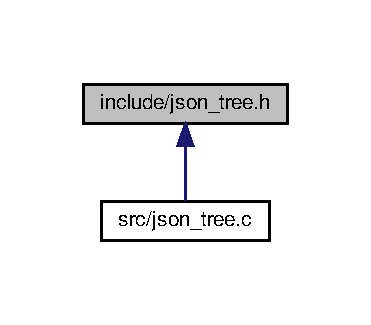
\includegraphics[width=178pt]{json__tree_8h__dep__incl}
\end{center}
\end{figure}
\subsection*{Data Structures}
\begin{DoxyCompactItemize}
\item 
struct \hyperlink{struct__json__pair}{\+\_\+json\+\_\+pair}
\item 
union \hyperlink{unionJsonValue}{Json\+Value}
\begin{DoxyCompactList}\small\item\em pour stocker \char`\"{}value\char`\"{} \end{DoxyCompactList}\item 
struct \hyperlink{struct__json__value__container}{\+\_\+json\+\_\+value\+\_\+container}
\item 
struct \hyperlink{struct__json__object}{\+\_\+json\+\_\+object}
\item 
struct \hyperlink{struct__json__array}{\+\_\+json\+\_\+array}
\end{DoxyCompactItemize}
\subsection*{Macros}
\begin{DoxyCompactItemize}
\item 
\mbox{\Hypertarget{json__tree_8h_af4d0262661fb41a7a3e83eaaa0cde01d}\label{json__tree_8h_af4d0262661fb41a7a3e83eaaa0cde01d}} 
\#define {\bfseries C\+S\+T\+E\+\_\+\+J\+S\+O\+N\+\_\+\+N\+U\+LL}~2
\item 
\mbox{\Hypertarget{json__tree_8h_a52c777ff15f7f751e41e41e7f3f91fbb}\label{json__tree_8h_a52c777ff15f7f751e41e41e7f3f91fbb}} 
\#define {\bfseries C\+S\+T\+E\+\_\+\+J\+S\+O\+N\+\_\+\+T\+R\+UE}~1
\item 
\mbox{\Hypertarget{json__tree_8h_a4a64518555ef089bda8ae9def554aa3e}\label{json__tree_8h_a4a64518555ef089bda8ae9def554aa3e}} 
\#define {\bfseries C\+S\+T\+E\+\_\+\+J\+S\+O\+N\+\_\+\+F\+A\+L\+SE}~0
\end{DoxyCompactItemize}
\subsection*{Typedefs}
\begin{DoxyCompactItemize}
\item 
\mbox{\Hypertarget{json__tree_8h_ae67ac47c44d822409d979fce1b82d262}\label{json__tree_8h_ae67ac47c44d822409d979fce1b82d262}} 
typedef struct \hyperlink{struct__json__pair}{\+\_\+json\+\_\+pair} {\bfseries Json\+Pair}
\item 
\mbox{\Hypertarget{json__tree_8h_a4240fa9f317a2e54e34c73cc42f9f4ed}\label{json__tree_8h_a4240fa9f317a2e54e34c73cc42f9f4ed}} 
typedef enum \hyperlink{json__tree_8h_a5de71900664e9c2b31ef59a9352f0d28}{\+\_\+value\+\_\+type} {\bfseries Value\+Type}
\item 
\mbox{\Hypertarget{json__tree_8h_a6e8f0dbaec21e3776411e7f525f42d12}\label{json__tree_8h_a6e8f0dbaec21e3776411e7f525f42d12}} 
typedef struct \hyperlink{struct__json__value__container}{\+\_\+json\+\_\+value\+\_\+container} {\bfseries Json\+Value\+Container}
\item 
\mbox{\Hypertarget{json__tree_8h_a0beac496a571658774a814b486e772e1}\label{json__tree_8h_a0beac496a571658774a814b486e772e1}} 
typedef struct \hyperlink{struct__json__object}{\+\_\+json\+\_\+object} {\bfseries Json\+Object}
\item 
\mbox{\Hypertarget{json__tree_8h_a1b93cc6238d7024ba2ff8e83ad88e28f}\label{json__tree_8h_a1b93cc6238d7024ba2ff8e83ad88e28f}} 
typedef struct \hyperlink{struct__json__array}{\+\_\+json\+\_\+array} {\bfseries Json\+Array}
\end{DoxyCompactItemize}
\subsection*{Enumerations}
\begin{DoxyCompactItemize}
\item 
enum \hyperlink{json__tree_8h_a5de71900664e9c2b31ef59a9352f0d28}{\+\_\+value\+\_\+type} \{ \newline
{\bfseries string}, 
{\bfseries integer}, 
{\bfseries real}, 
{\bfseries object}, 
\newline
{\bfseries array}, 
\hyperlink{json__tree_8h_a5de71900664e9c2b31ef59a9352f0d28a995640a12d5339aabee76a933fb5f519}{constant}
 \}
\end{DoxyCompactItemize}
\subsection*{Functions}
\begin{DoxyCompactItemize}
\item 
\hyperlink{structJsonArray}{Json\+Array} $\ast$ \hyperlink{json__tree_8h_a64a23e508691b4752f9d3423ce7f44cf}{Create\+Json\+Array} ()
\begin{DoxyCompactList}\small\item\em creation en memoire d\textquotesingle{}un \hyperlink{structJsonArray}{Json\+Array} \end{DoxyCompactList}\item 
\mbox{\Hypertarget{json__tree_8h_ae1f0848cee2a75adc68951d7f4e0db94}\label{json__tree_8h_ae1f0848cee2a75adc68951d7f4e0db94}} 
int {\bfseries Insert\+Json\+Array} (\hyperlink{structJsonArray}{Json\+Array} $\ast$\+\_\+array, \hyperlink{structJsonValueContainer}{Json\+Value\+Container} $\ast$\+\_\+value\+Container, const unsigned int \+\_\+position)
\item 
\mbox{\Hypertarget{json__tree_8h_a61372b2f4a3eb734f752159f6265940d}\label{json__tree_8h_a61372b2f4a3eb734f752159f6265940d}} 
int {\bfseries Delete\+Json\+Array} (\hyperlink{structJsonArray}{Json\+Array} $\ast$$\ast$\+\_\+array)
\item 
\mbox{\Hypertarget{json__tree_8h_a30b5080b3f6aba1bbf430aac34d912f7}\label{json__tree_8h_a30b5080b3f6aba1bbf430aac34d912f7}} 
char $\ast$ {\bfseries Print\+Json\+Array} (const \hyperlink{structJsonArray}{Json\+Array} $\ast$\+\_\+array)
\item 
\mbox{\Hypertarget{json__tree_8h_a60f3e947d378f0d1513a6a2495110e0f}\label{json__tree_8h_a60f3e947d378f0d1513a6a2495110e0f}} 
char $\ast$ {\bfseries Print\+Dot\+Json\+Array} (const \hyperlink{structJsonArray}{Json\+Array} $\ast$\+\_\+array)
\item 
\hyperlink{structJsonObject}{Json\+Object} $\ast$ \hyperlink{json__tree_8h_af7af287d13cd208992c31d69f838c816}{Create\+Json\+Object} ()
\begin{DoxyCompactList}\small\item\em construit un \hyperlink{structJsonObject}{Json\+Object} vide \end{DoxyCompactList}\item 
\mbox{\Hypertarget{json__tree_8h_add92f2aba1fffe0af85073527c95fc0e}\label{json__tree_8h_add92f2aba1fffe0af85073527c95fc0e}} 
int {\bfseries Insert\+Json\+Object} (\hyperlink{structJsonObject}{Json\+Object} $\ast$\+\_\+object, \hyperlink{structJsonPair}{Json\+Pair} $\ast$\+\_\+pair)
\item 
\mbox{\Hypertarget{json__tree_8h_af308a2f032f23582b09b7a0238f8f268}\label{json__tree_8h_af308a2f032f23582b09b7a0238f8f268}} 
\hyperlink{structJsonValueContainer}{Json\+Value\+Container} $\ast$ {\bfseries Get\+Json\+Value\+Container} (const \hyperlink{structJsonObject}{Json\+Object} $\ast$\+\_\+object, const char $\ast$\+\_\+string)
\item 
\mbox{\Hypertarget{json__tree_8h_ab9fcb0ea6aba690197eeaa9170d6e279}\label{json__tree_8h_ab9fcb0ea6aba690197eeaa9170d6e279}} 
int {\bfseries Delete\+Json\+Object} (\hyperlink{structJsonObject}{Json\+Object} $\ast$$\ast$\+\_\+object)
\item 
\mbox{\Hypertarget{json__tree_8h_ae153464704693dc8283f34792b4c0a2e}\label{json__tree_8h_ae153464704693dc8283f34792b4c0a2e}} 
char $\ast$ {\bfseries Print\+Json\+Object} (const \hyperlink{structJsonObject}{Json\+Object} $\ast$\+\_\+object)
\item 
\mbox{\Hypertarget{json__tree_8h_a995ed6708039e3e415e5baf8d00ea62e}\label{json__tree_8h_a995ed6708039e3e415e5baf8d00ea62e}} 
char $\ast$ {\bfseries Print\+Dot\+Json\+Object} (const \hyperlink{structJsonObject}{Json\+Object} $\ast$\+\_\+object, int \+\_\+id, int \+\_\+id\+Parent)
\item 
\hyperlink{structJsonValueContainer}{Json\+Value\+Container} $\ast$ \hyperlink{json__tree_8h_a9bab288b17c70677b8c1d7619b2925fc}{Create\+Json\+Value\+Container} ()
\begin{DoxyCompactList}\small\item\em construit un \hyperlink{structJsonValueContainer}{Json\+Value\+Container} vide \end{DoxyCompactList}\item 
\mbox{\Hypertarget{json__tree_8h_a918da5f7ca94d6544f77bef2fb75c177}\label{json__tree_8h_a918da5f7ca94d6544f77bef2fb75c177}} 
void {\bfseries Update\+Json\+Value\+Container} (\hyperlink{structJsonValueContainer}{Json\+Value\+Container} $\ast$\+\_\+value\+Container, Value\+Type \+\_\+type, \hyperlink{unionJsonValue}{Json\+Value} \+\_\+value)
\item 
\mbox{\Hypertarget{json__tree_8h_a6d02f560a673f8f70aec2c88d8e32d2d}\label{json__tree_8h_a6d02f560a673f8f70aec2c88d8e32d2d}} 
int {\bfseries Delete\+Json\+Value\+Container} (\hyperlink{structJsonValueContainer}{Json\+Value\+Container} $\ast$$\ast$\+\_\+value\+Container)
\item 
\mbox{\Hypertarget{json__tree_8h_ac93a83ad1ed7f56dd9ecd83e5dfdbdb6}\label{json__tree_8h_ac93a83ad1ed7f56dd9ecd83e5dfdbdb6}} 
char $\ast$ {\bfseries Print\+Json\+Value\+Container} (const \hyperlink{structJsonValueContainer}{Json\+Value\+Container} $\ast$\+\_\+value\+Container)
\item 
\hyperlink{structJsonPair}{Json\+Pair} $\ast$ \hyperlink{json__tree_8h_ad88d80b56f7d04bea1de11917e34fa3d}{Create\+Json\+Pair} ()
\item 
\mbox{\Hypertarget{json__tree_8h_a028e96028bb843d57b69aecb42b50df1}\label{json__tree_8h_a028e96028bb843d57b69aecb42b50df1}} 
void {\bfseries Update\+Json\+Pair} (\hyperlink{structJsonPair}{Json\+Pair} $\ast$\+\_\+pair, char $\ast$\+\_\+string, \hyperlink{structJsonValueContainer}{Json\+Value\+Container} $\ast$\+\_\+value)
\item 
\mbox{\Hypertarget{json__tree_8h_abcd2910290251bc96cec45cf46d364b7}\label{json__tree_8h_abcd2910290251bc96cec45cf46d364b7}} 
int {\bfseries Delete\+Json\+Pair} (\hyperlink{structJsonPair}{Json\+Pair} $\ast$$\ast$\+\_\+pair)
\item 
\mbox{\Hypertarget{json__tree_8h_aa520ede60813d831e4d92fa2061ed0c4}\label{json__tree_8h_aa520ede60813d831e4d92fa2061ed0c4}} 
char $\ast$ {\bfseries Print\+Json\+Pair} (const \hyperlink{structJsonPair}{Json\+Pair} $\ast$\+\_\+pair)
\end{DoxyCompactItemize}


\subsection{Detailed Description}
implemente la mise en memoire d\textquotesingle{}un arbre json 

\begin{DoxyAuthor}{Author}
NM 
\end{DoxyAuthor}
\begin{DoxyVersion}{Version}
0.\+1 
\end{DoxyVersion}
\begin{DoxyDate}{Date}
06.\+12.\+2014 
\end{DoxyDate}


\subsection{Enumeration Type Documentation}
\mbox{\Hypertarget{json__tree_8h_a5de71900664e9c2b31ef59a9352f0d28}\label{json__tree_8h_a5de71900664e9c2b31ef59a9352f0d28}} 
\index{json\+\_\+tree.\+h@{json\+\_\+tree.\+h}!\+\_\+value\+\_\+type@{\+\_\+value\+\_\+type}}
\index{\+\_\+value\+\_\+type@{\+\_\+value\+\_\+type}!json\+\_\+tree.\+h@{json\+\_\+tree.\+h}}
\subsubsection{\texorpdfstring{\+\_\+value\+\_\+type}{\_value\_type}}
{\footnotesize\ttfamily enum \hyperlink{json__tree_8h_a5de71900664e9c2b31ef59a9352f0d28}{\+\_\+value\+\_\+type}}

\begin{DoxyEnumFields}{Enumerator}
\raisebox{\heightof{T}}[0pt][0pt]{\index{constant@{constant}!json\+\_\+tree.\+h@{json\+\_\+tree.\+h}}\index{json\+\_\+tree.\+h@{json\+\_\+tree.\+h}!constant@{constant}}}\mbox{\Hypertarget{json__tree_8h_a5de71900664e9c2b31ef59a9352f0d28a995640a12d5339aabee76a933fb5f519}\label{json__tree_8h_a5de71900664e9c2b31ef59a9352f0d28a995640a12d5339aabee76a933fb5f519}} 
constant&pour true, false et null \\
\hline

\end{DoxyEnumFields}


\subsection{Function Documentation}
\mbox{\Hypertarget{json__tree_8h_a64a23e508691b4752f9d3423ce7f44cf}\label{json__tree_8h_a64a23e508691b4752f9d3423ce7f44cf}} 
\index{json\+\_\+tree.\+h@{json\+\_\+tree.\+h}!Create\+Json\+Array@{Create\+Json\+Array}}
\index{Create\+Json\+Array@{Create\+Json\+Array}!json\+\_\+tree.\+h@{json\+\_\+tree.\+h}}
\subsubsection{\texorpdfstring{Create\+Json\+Array()}{CreateJsonArray()}}
{\footnotesize\ttfamily \hyperlink{structJsonArray}{Json\+Array}$\ast$ Create\+Json\+Array (\begin{DoxyParamCaption}{ }\end{DoxyParamCaption})}



creation en memoire d\textquotesingle{}un \hyperlink{structJsonArray}{Json\+Array} 

\begin{DoxyReturn}{Returns}
Json\+Array$\ast$ 
\end{DoxyReturn}
\mbox{\Hypertarget{json__tree_8h_af7af287d13cd208992c31d69f838c816}\label{json__tree_8h_af7af287d13cd208992c31d69f838c816}} 
\index{json\+\_\+tree.\+h@{json\+\_\+tree.\+h}!Create\+Json\+Object@{Create\+Json\+Object}}
\index{Create\+Json\+Object@{Create\+Json\+Object}!json\+\_\+tree.\+h@{json\+\_\+tree.\+h}}
\subsubsection{\texorpdfstring{Create\+Json\+Object()}{CreateJsonObject()}}
{\footnotesize\ttfamily \hyperlink{structJsonObject}{Json\+Object}$\ast$ Create\+Json\+Object (\begin{DoxyParamCaption}{ }\end{DoxyParamCaption})}



construit un \hyperlink{structJsonObject}{Json\+Object} vide 

\begin{DoxyReturn}{Returns}
\hyperlink{structJsonObject}{Json\+Object} $\ast$ 
\end{DoxyReturn}
\mbox{\Hypertarget{json__tree_8h_ad88d80b56f7d04bea1de11917e34fa3d}\label{json__tree_8h_ad88d80b56f7d04bea1de11917e34fa3d}} 
\index{json\+\_\+tree.\+h@{json\+\_\+tree.\+h}!Create\+Json\+Pair@{Create\+Json\+Pair}}
\index{Create\+Json\+Pair@{Create\+Json\+Pair}!json\+\_\+tree.\+h@{json\+\_\+tree.\+h}}
\subsubsection{\texorpdfstring{Create\+Json\+Pair()}{CreateJsonPair()}}
{\footnotesize\ttfamily \hyperlink{structJsonPair}{Json\+Pair}$\ast$ Create\+Json\+Pair (\begin{DoxyParamCaption}{ }\end{DoxyParamCaption})}


\begin{DoxyParams}{Parameters}
{\em } & \\
\hline
\end{DoxyParams}
\mbox{\Hypertarget{json__tree_8h_a9bab288b17c70677b8c1d7619b2925fc}\label{json__tree_8h_a9bab288b17c70677b8c1d7619b2925fc}} 
\index{json\+\_\+tree.\+h@{json\+\_\+tree.\+h}!Create\+Json\+Value\+Container@{Create\+Json\+Value\+Container}}
\index{Create\+Json\+Value\+Container@{Create\+Json\+Value\+Container}!json\+\_\+tree.\+h@{json\+\_\+tree.\+h}}
\subsubsection{\texorpdfstring{Create\+Json\+Value\+Container()}{CreateJsonValueContainer()}}
{\footnotesize\ttfamily \hyperlink{structJsonValueContainer}{Json\+Value\+Container}$\ast$ Create\+Json\+Value\+Container (\begin{DoxyParamCaption}{ }\end{DoxyParamCaption})}



construit un \hyperlink{structJsonValueContainer}{Json\+Value\+Container} vide 


\begin{DoxyParams}{Parameters}
{\em } & \\
\hline
\end{DoxyParams}

\hypertarget{pile_8h}{}\section{include/pile.h File Reference}
\label{pile_8h}\index{include/pile.\+h@{include/pile.\+h}}


gestion d\textquotesingle{}une pile  


This graph shows which files directly or indirectly include this file\+:\nopagebreak
\begin{figure}[H]
\begin{center}
\leavevmode
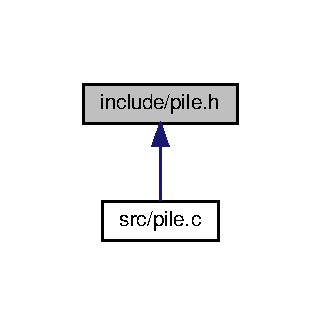
\includegraphics[width=154pt]{pile_8h__dep__incl}
\end{center}
\end{figure}
\subsection*{Data Structures}
\begin{DoxyCompactItemize}
\item 
struct \hyperlink{structTIntPile}{T\+Int\+Pile}
\begin{DoxyCompactList}\small\item\em structure contenant une pile d\textquotesingle{}entiers \end{DoxyCompactList}\item 
struct \hyperlink{structTVoidPile}{T\+Void\+Pile}
\begin{DoxyCompactList}\small\item\em structure contenant une pile de pointeur void $\ast$ \end{DoxyCompactList}\end{DoxyCompactItemize}
\subsection*{Functions}
\begin{DoxyCompactItemize}
\item 
\mbox{\Hypertarget{pile_8h_a401766bcab875227f3fe0b4a2c314d9b}\label{pile_8h_a401766bcab875227f3fe0b4a2c314d9b}} 
\hyperlink{structTIntPile}{T\+Int\+Pile} $\ast$ {\bfseries init\+Int\+Pile} ()
\item 
void \hyperlink{pile_8h_a4d8c955ed39c0e02ff16c2583240b4c3}{delete\+Int\+Pile} (\hyperlink{structTIntPile}{T\+Int\+Pile} $\ast$$\ast$\+\_\+pile)
\begin{DoxyCompactList}\small\item\em efface la memoire occupe par la pile \end{DoxyCompactList}\item 
void \hyperlink{pile_8h_a525764cab275369f56d230e3a911cfb6}{print\+Int\+Pile} (\hyperlink{structTIntPile}{T\+Int\+Pile} $\ast$\+\_\+pile)
\begin{DoxyCompactList}\small\item\em affichage du contenu d\textquotesingle{}une pile \end{DoxyCompactList}\item 
void \hyperlink{pile_8h_aca7a8bc8998e15add0598f09a65afa97}{empiler\+Int} (\hyperlink{structTIntPile}{T\+Int\+Pile} $\ast$\+\_\+pile, int \+\_\+val)
\begin{DoxyCompactList}\small\item\em empiler un entier sur la pile, si la zone memoire reservee n\textquotesingle{}est pas suffisante, celle-\/ci est etendue \end{DoxyCompactList}\item 
int \hyperlink{pile_8h_a823ba490199cf04477b74b070e22f3be}{depiler\+Int} (\hyperlink{structTIntPile}{T\+Int\+Pile} $\ast$\+\_\+pile)
\begin{DoxyCompactList}\small\item\em dépiler un entier \end{DoxyCompactList}\item 
int \hyperlink{pile_8h_a8f2c03c053b2b6b9540eeeff20baa086}{sommet\+Int} (\hyperlink{structTIntPile}{T\+Int\+Pile} $\ast$\+\_\+pile)
\begin{DoxyCompactList}\small\item\em renvoie la valeur du sommet (sans depiler) \end{DoxyCompactList}\item 
\hyperlink{structTVoidPile}{T\+Void\+Pile} $\ast$ \hyperlink{pile_8h_a7aa48e45fedc96e4fbcc0b0c64e6b38b}{init\+Void\+Pile} ()
\begin{DoxyCompactList}\small\item\em fonction qui initialise une pile de pointeur void $\ast$ \end{DoxyCompactList}\item 
void \hyperlink{pile_8h_a1471f95a65ffd6cc6f3ddeccde2ab327}{delete\+Void\+Pile} (\hyperlink{structTVoidPile}{T\+Void\+Pile} $\ast$$\ast$\+\_\+pile)
\begin{DoxyCompactList}\small\item\em libere la memoire occupee par la pile \end{DoxyCompactList}\item 
void \hyperlink{pile_8h_aa2185907bdfe2791481e174384c41253}{print\+Void\+Pile} (\hyperlink{structTVoidPile}{T\+Void\+Pile} $\ast$\+\_\+pile)
\begin{DoxyCompactList}\small\item\em affichage de la pile (comme on ne connait pas les type des elements empiles, on affiche les adresses de tous les pointeurs empiles) \end{DoxyCompactList}\item 
void \hyperlink{pile_8h_ade2214f96e200aafa5ef341103943de6}{empiler\+Void} (\hyperlink{structTVoidPile}{T\+Void\+Pile} $\ast$\+\_\+pile, void $\ast$\+\_\+val)
\begin{DoxyCompactList}\small\item\em empile un void $\ast$ \end{DoxyCompactList}\item 
void $\ast$ \hyperlink{pile_8h_a43e95f3256f3c25c7a8e818c1ee9227d}{depiler\+Void} (\hyperlink{structTVoidPile}{T\+Void\+Pile} $\ast$\+\_\+pile)
\begin{DoxyCompactList}\small\item\em dépiler un élément de type void $\ast$ \end{DoxyCompactList}\item 
void $\ast$ \hyperlink{pile_8h_ab993675f3a0e701efc8f0cb702640eea}{sommet\+Void} (\hyperlink{structTVoidPile}{T\+Void\+Pile} $\ast$\+\_\+pile)
\begin{DoxyCompactList}\small\item\em obtenir la valeur du sommet de type void $\ast$ \end{DoxyCompactList}\end{DoxyCompactItemize}


\subsection{Detailed Description}
gestion d\textquotesingle{}une pile 

\begin{DoxyAuthor}{Author}
NM 
\end{DoxyAuthor}
\begin{DoxyVersion}{Version}
0.\+1 
\end{DoxyVersion}
\begin{DoxyDate}{Date}
11/12/2015 
\end{DoxyDate}


\subsection{Function Documentation}
\mbox{\Hypertarget{pile_8h_a4d8c955ed39c0e02ff16c2583240b4c3}\label{pile_8h_a4d8c955ed39c0e02ff16c2583240b4c3}} 
\index{pile.\+h@{pile.\+h}!delete\+Int\+Pile@{delete\+Int\+Pile}}
\index{delete\+Int\+Pile@{delete\+Int\+Pile}!pile.\+h@{pile.\+h}}
\subsubsection{\texorpdfstring{delete\+Int\+Pile()}{deleteIntPile()}}
{\footnotesize\ttfamily void delete\+Int\+Pile (\begin{DoxyParamCaption}\item[{\hyperlink{structTIntPile}{T\+Int\+Pile} $\ast$$\ast$}]{\+\_\+pile }\end{DoxyParamCaption})}



efface la memoire occupe par la pile 


\begin{DoxyParams}{Parameters}
{\em } & \\
\hline
\end{DoxyParams}
\mbox{\Hypertarget{pile_8h_a1471f95a65ffd6cc6f3ddeccde2ab327}\label{pile_8h_a1471f95a65ffd6cc6f3ddeccde2ab327}} 
\index{pile.\+h@{pile.\+h}!delete\+Void\+Pile@{delete\+Void\+Pile}}
\index{delete\+Void\+Pile@{delete\+Void\+Pile}!pile.\+h@{pile.\+h}}
\subsubsection{\texorpdfstring{delete\+Void\+Pile()}{deleteVoidPile()}}
{\footnotesize\ttfamily void delete\+Void\+Pile (\begin{DoxyParamCaption}\item[{\hyperlink{structTVoidPile}{T\+Void\+Pile} $\ast$$\ast$}]{\+\_\+pile }\end{DoxyParamCaption})}



libere la memoire occupee par la pile 


\begin{DoxyParams}[1]{Parameters}
\mbox{\tt in}  & {\em \+\_\+pile} & \+: adresse du pointeur sur la pile a liberer \\
\hline
\end{DoxyParams}
\begin{DoxyReturn}{Returns}
neant 
\end{DoxyReturn}
\mbox{\Hypertarget{pile_8h_a823ba490199cf04477b74b070e22f3be}\label{pile_8h_a823ba490199cf04477b74b070e22f3be}} 
\index{pile.\+h@{pile.\+h}!depiler\+Int@{depiler\+Int}}
\index{depiler\+Int@{depiler\+Int}!pile.\+h@{pile.\+h}}
\subsubsection{\texorpdfstring{depiler\+Int()}{depilerInt()}}
{\footnotesize\ttfamily int depiler\+Int (\begin{DoxyParamCaption}\item[{\hyperlink{structTIntPile}{T\+Int\+Pile} $\ast$}]{\+\_\+pile }\end{DoxyParamCaption})}



dépiler un entier 


\begin{DoxyParams}[1]{Parameters}
\mbox{\tt in}  & {\em \+\_\+pile} & \+: la pile a depiler \\
\hline
\end{DoxyParams}
\begin{DoxyReturn}{Returns}
l\textquotesingle{}entier en sommet de pile (0 si la pile est vide) 
\end{DoxyReturn}
\mbox{\Hypertarget{pile_8h_a43e95f3256f3c25c7a8e818c1ee9227d}\label{pile_8h_a43e95f3256f3c25c7a8e818c1ee9227d}} 
\index{pile.\+h@{pile.\+h}!depiler\+Void@{depiler\+Void}}
\index{depiler\+Void@{depiler\+Void}!pile.\+h@{pile.\+h}}
\subsubsection{\texorpdfstring{depiler\+Void()}{depilerVoid()}}
{\footnotesize\ttfamily void$\ast$ depiler\+Void (\begin{DoxyParamCaption}\item[{\hyperlink{structTVoidPile}{T\+Void\+Pile} $\ast$}]{\+\_\+pile }\end{DoxyParamCaption})}



dépiler un élément de type void $\ast$ 


\begin{DoxyParams}[1]{Parameters}
\mbox{\tt in}  & {\em \+\_\+pile} & \+: pile a utiliser \\
\hline
\end{DoxyParams}
\begin{DoxyReturn}{Returns}
pointeur sur void (0 si la pile est vide) 
\end{DoxyReturn}
\mbox{\Hypertarget{pile_8h_aca7a8bc8998e15add0598f09a65afa97}\label{pile_8h_aca7a8bc8998e15add0598f09a65afa97}} 
\index{pile.\+h@{pile.\+h}!empiler\+Int@{empiler\+Int}}
\index{empiler\+Int@{empiler\+Int}!pile.\+h@{pile.\+h}}
\subsubsection{\texorpdfstring{empiler\+Int()}{empilerInt()}}
{\footnotesize\ttfamily void empiler\+Int (\begin{DoxyParamCaption}\item[{\hyperlink{structTIntPile}{T\+Int\+Pile} $\ast$}]{\+\_\+pile,  }\item[{int}]{\+\_\+val }\end{DoxyParamCaption})}



empiler un entier sur la pile, si la zone memoire reservee n\textquotesingle{}est pas suffisante, celle-\/ci est etendue 


\begin{DoxyParams}{Parameters}
{\em } & \\
\hline
\end{DoxyParams}
\mbox{\Hypertarget{pile_8h_ade2214f96e200aafa5ef341103943de6}\label{pile_8h_ade2214f96e200aafa5ef341103943de6}} 
\index{pile.\+h@{pile.\+h}!empiler\+Void@{empiler\+Void}}
\index{empiler\+Void@{empiler\+Void}!pile.\+h@{pile.\+h}}
\subsubsection{\texorpdfstring{empiler\+Void()}{empilerVoid()}}
{\footnotesize\ttfamily void empiler\+Void (\begin{DoxyParamCaption}\item[{\hyperlink{structTVoidPile}{T\+Void\+Pile} $\ast$}]{\+\_\+pile,  }\item[{void $\ast$}]{\+\_\+val }\end{DoxyParamCaption})}



empile un void $\ast$ 


\begin{DoxyParams}{Parameters}
{\em } & \\
\hline
\end{DoxyParams}
\mbox{\Hypertarget{pile_8h_a7aa48e45fedc96e4fbcc0b0c64e6b38b}\label{pile_8h_a7aa48e45fedc96e4fbcc0b0c64e6b38b}} 
\index{pile.\+h@{pile.\+h}!init\+Void\+Pile@{init\+Void\+Pile}}
\index{init\+Void\+Pile@{init\+Void\+Pile}!pile.\+h@{pile.\+h}}
\subsubsection{\texorpdfstring{init\+Void\+Pile()}{initVoidPile()}}
{\footnotesize\ttfamily \hyperlink{structTVoidPile}{T\+Void\+Pile}$\ast$ init\+Void\+Pile (\begin{DoxyParamCaption}{ }\end{DoxyParamCaption})}



fonction qui initialise une pile de pointeur void $\ast$ 

pile de void $\ast$ -\/-\/-\/-\/-\/-\/-\/-\/-\/-\/-\/-\/-\/-\/-\/-\/-\/-\/-\/-\/-\/-\/-\/-\/-\/-\/-\/-\/-\/-\/-\/-\/-\/-\/-\/-\/-\/-\/-\/-\/-\/-\/-\/-\/-\/------

\begin{DoxyReturn}{Returns}
pointeur sur une pile \hyperlink{structTVoidPile}{T\+Void\+Pile} 
\end{DoxyReturn}
\mbox{\Hypertarget{pile_8h_a525764cab275369f56d230e3a911cfb6}\label{pile_8h_a525764cab275369f56d230e3a911cfb6}} 
\index{pile.\+h@{pile.\+h}!print\+Int\+Pile@{print\+Int\+Pile}}
\index{print\+Int\+Pile@{print\+Int\+Pile}!pile.\+h@{pile.\+h}}
\subsubsection{\texorpdfstring{print\+Int\+Pile()}{printIntPile()}}
{\footnotesize\ttfamily void print\+Int\+Pile (\begin{DoxyParamCaption}\item[{\hyperlink{structTIntPile}{T\+Int\+Pile} $\ast$}]{\+\_\+pile }\end{DoxyParamCaption})}



affichage du contenu d\textquotesingle{}une pile 


\begin{DoxyParams}[1]{Parameters}
\mbox{\tt in}  & {\em \+\_\+pile} & \+: la pile a afficher \\
\hline
\end{DoxyParams}
\begin{DoxyReturn}{Returns}
neant 
\end{DoxyReturn}
\mbox{\Hypertarget{pile_8h_aa2185907bdfe2791481e174384c41253}\label{pile_8h_aa2185907bdfe2791481e174384c41253}} 
\index{pile.\+h@{pile.\+h}!print\+Void\+Pile@{print\+Void\+Pile}}
\index{print\+Void\+Pile@{print\+Void\+Pile}!pile.\+h@{pile.\+h}}
\subsubsection{\texorpdfstring{print\+Void\+Pile()}{printVoidPile()}}
{\footnotesize\ttfamily void print\+Void\+Pile (\begin{DoxyParamCaption}\item[{\hyperlink{structTVoidPile}{T\+Void\+Pile} $\ast$}]{\+\_\+pile }\end{DoxyParamCaption})}



affichage de la pile (comme on ne connait pas les type des elements empiles, on affiche les adresses de tous les pointeurs empiles) 


\begin{DoxyParams}[1]{Parameters}
\mbox{\tt in}  & {\em \+\_\+pile} & \+: pile a afficher \\
\hline
\end{DoxyParams}
\begin{DoxyReturn}{Returns}
neant 
\end{DoxyReturn}
\mbox{\Hypertarget{pile_8h_a8f2c03c053b2b6b9540eeeff20baa086}\label{pile_8h_a8f2c03c053b2b6b9540eeeff20baa086}} 
\index{pile.\+h@{pile.\+h}!sommet\+Int@{sommet\+Int}}
\index{sommet\+Int@{sommet\+Int}!pile.\+h@{pile.\+h}}
\subsubsection{\texorpdfstring{sommet\+Int()}{sommetInt()}}
{\footnotesize\ttfamily int sommet\+Int (\begin{DoxyParamCaption}\item[{\hyperlink{structTIntPile}{T\+Int\+Pile} $\ast$}]{\+\_\+pile }\end{DoxyParamCaption})}



renvoie la valeur du sommet (sans depiler) 


\begin{DoxyParams}[1]{Parameters}
\mbox{\tt in}  & {\em \+\_\+pile} & \+: la pile a utiliser \\
\hline
\end{DoxyParams}
\begin{DoxyReturn}{Returns}
l\textquotesingle{}entier en sommet de pile (0 si la pile est vide) 
\end{DoxyReturn}
\mbox{\Hypertarget{pile_8h_ab993675f3a0e701efc8f0cb702640eea}\label{pile_8h_ab993675f3a0e701efc8f0cb702640eea}} 
\index{pile.\+h@{pile.\+h}!sommet\+Void@{sommet\+Void}}
\index{sommet\+Void@{sommet\+Void}!pile.\+h@{pile.\+h}}
\subsubsection{\texorpdfstring{sommet\+Void()}{sommetVoid()}}
{\footnotesize\ttfamily void$\ast$ sommet\+Void (\begin{DoxyParamCaption}\item[{\hyperlink{structTVoidPile}{T\+Void\+Pile} $\ast$}]{\+\_\+pile }\end{DoxyParamCaption})}



obtenir la valeur du sommet de type void $\ast$ 


\begin{DoxyParams}[1]{Parameters}
\mbox{\tt in}  & {\em \+\_\+pile} & \+: pile a utiliser pour lire le sommet \\
\hline
\end{DoxyParams}
\begin{DoxyReturn}{Returns}
la valeur void $\ast$ du sommet (0 si la pile est vide) 
\end{DoxyReturn}

\hypertarget{tp2__lex_8h}{}\section{include/tp2\+\_\+lex.h File Reference}
\label{tp2__lex_8h}\index{include/tp2\+\_\+lex.\+h@{include/tp2\+\_\+lex.\+h}}


analyseur lexical pour le langage J\+S\+ON  


This graph shows which files directly or indirectly include this file\+:\nopagebreak
\begin{figure}[H]
\begin{center}
\leavevmode
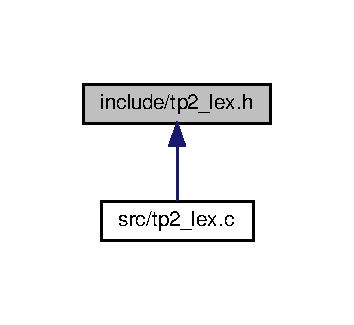
\includegraphics[width=170pt]{tp2__lex_8h__dep__incl}
\end{center}
\end{figure}
\subsection*{Data Structures}
\begin{DoxyCompactItemize}
\item 
union \hyperlink{structTSymbole}{T\+Symbole}
\begin{DoxyCompactList}\small\item\em union permettant de manipuler un entier/reel/chaine pour la table des symboles \end{DoxyCompactList}\item 
struct \hyperlink{structTLex}{T\+Lex}
\begin{DoxyCompactList}\small\item\em structure contenant tous les parametres/donnees pour l\textquotesingle{}analyse lexicale \end{DoxyCompactList}\end{DoxyCompactItemize}
\subsection*{Macros}
\begin{DoxyCompactItemize}
\item 
\#define \hyperlink{tp2__lex_8h_a1c1d6b9a4119ed60f57af0732bbc7ac4}{J\+S\+O\+N\+\_\+\+L\+E\+X\+\_\+\+E\+R\+R\+OR}~-\/1
\item 
\#define \hyperlink{tp2__lex_8h_a172a7e23fb0ac9f8ce19bee485090de7}{J\+S\+O\+N\+\_\+\+T\+R\+UE}~1
\item 
\#define \hyperlink{tp2__lex_8h_a8944b24b93d4a397aa5748a5f6048d5b}{J\+S\+O\+N\+\_\+\+F\+A\+L\+SE}~2
\item 
\#define \hyperlink{tp2__lex_8h_a47153ed2f7bd07cabffd495e4a18839f}{J\+S\+O\+N\+\_\+\+N\+U\+LL}~3
\item 
\#define \hyperlink{tp2__lex_8h_a3b936ae16a984c94b371ed1e8bc74465}{J\+S\+O\+N\+\_\+\+L\+CB}~4
\item 
\#define \hyperlink{tp2__lex_8h_a8505d4213a71673ca62aa1e799e4333c}{J\+S\+O\+N\+\_\+\+R\+CB}~5
\item 
\#define \hyperlink{tp2__lex_8h_afc6172b33cb8b8fc84d963789eaf6a09}{J\+S\+O\+N\+\_\+\+LB}~6
\item 
\#define \hyperlink{tp2__lex_8h_ab08abc8e5d15d3b8c0be234acc188c21}{J\+S\+O\+N\+\_\+\+RB}~7
\item 
\#define \hyperlink{tp2__lex_8h_a397f200787ea6874ad6ab9e489f6f3a5}{J\+S\+O\+N\+\_\+\+C\+O\+M\+MA}~8
\item 
\#define \hyperlink{tp2__lex_8h_a6ba5aa52b05c03ce1b467e69dac56732}{J\+S\+O\+N\+\_\+\+C\+O\+L\+ON}~9
\item 
\#define \hyperlink{tp2__lex_8h_adea584ac98210649e2edf68941091356}{J\+S\+O\+N\+\_\+\+S\+T\+R\+I\+NG}~10
\item 
\#define \hyperlink{tp2__lex_8h_a85e4eb9195094b4e49d1f61755305bf7}{J\+S\+O\+N\+\_\+\+I\+N\+T\+\_\+\+N\+U\+M\+B\+ER}~11
\item 
\#define \hyperlink{tp2__lex_8h_a48c8d34a4f14411618cd63b06b0e822d}{J\+S\+O\+N\+\_\+\+R\+E\+A\+L\+\_\+\+N\+U\+M\+B\+ER}~12
\end{DoxyCompactItemize}
\subsection*{Functions}
\begin{DoxyCompactItemize}
\item 
int \hyperlink{tp2__lex_8h_a9869519009e3b965c6401e67261f6c43}{is\+Sep} (const char \+\_\+symb)
\begin{DoxyCompactList}\small\item\em fonction qui teste si un symbole fait partie des separateurs \end{DoxyCompactList}\item 
\hyperlink{structTLex}{T\+Lex} $\ast$ \hyperlink{tp2__lex_8h_a4a617721154587a6ea133054e7d3c55c}{init\+Lex\+Data} (char $\ast$\+\_\+data)
\begin{DoxyCompactList}\small\item\em fonction qui reserve la memoire et initialise les donnees pour l\textquotesingle{}analyseur lexical \end{DoxyCompactList}\item 
void \hyperlink{tp2__lex_8h_a66ac3a0b39b824a8e72654633945a95f}{delete\+Lex\+Data} (\hyperlink{structTLex}{T\+Lex} $\ast$$\ast$\+\_\+lex\+Data)
\begin{DoxyCompactList}\small\item\em fonction qui supprime de la memoire les donnees pour l\textquotesingle{}analyseur lexical \end{DoxyCompactList}\item 
void \hyperlink{tp2__lex_8h_a5cad73df0d00e5735e16356504a923b1}{print\+Lex\+Data} (\hyperlink{structTLex}{T\+Lex} $\ast$\+\_\+lex\+Data)
\begin{DoxyCompactList}\small\item\em fonction qui affiche les donnees pour l\textquotesingle{}analyseur lexical \end{DoxyCompactList}\item 
int \hyperlink{tp2__lex_8h_afed09d4c5ae5433e332256c311411bb6}{change\+Table\+Symbole\+Size} (\hyperlink{structTLex}{T\+Lex} $\ast$\+\_\+lex\+Data)
\begin{DoxyCompactList}\small\item\em Fonction qui incrémente le nombre de symbole de la table des symbole et augmente sa taille. \end{DoxyCompactList}\item 
void \hyperlink{tp2__lex_8h_a769d490ddf9b2cae334051946a61573b}{add\+Int\+Symbol\+To\+Lex\+Data} (\hyperlink{structTLex}{T\+Lex} $\ast$\+\_\+lex\+Data, const int \+\_\+val)
\begin{DoxyCompactList}\small\item\em fonction qui ajoute un symbole entier a la table des symboles \end{DoxyCompactList}\item 
void \hyperlink{tp2__lex_8h_a42504307caaa42184de9dd79b180b946}{add\+Real\+Symbol\+To\+Lex\+Data} (\hyperlink{structTLex}{T\+Lex} $\ast$\+\_\+lex\+Data, const float \+\_\+val)
\begin{DoxyCompactList}\small\item\em fonction qui ajoute un symbole reel a la table des symboles \end{DoxyCompactList}\item 
void \hyperlink{tp2__lex_8h_acc16ce9abf0d176fbe754943171f5c4e}{add\+String\+Symbol\+To\+Lex\+Data} (\hyperlink{structTLex}{T\+Lex} $\ast$\+\_\+lex\+Data, char $\ast$\+\_\+val)
\begin{DoxyCompactList}\small\item\em fonction qui ajoute une chaine de caracteres a la table des symboles \end{DoxyCompactList}\item 
\mbox{\Hypertarget{tp2__lex_8h_a4f39d3deacca77d7b4cf543101da84a6}\label{tp2__lex_8h_a4f39d3deacca77d7b4cf543101da84a6}} 
int {\bfseries lex} (\hyperlink{structTLex}{T\+Lex} $\ast$\+\_\+lex\+Data)
\end{DoxyCompactItemize}


\subsection{Detailed Description}
analyseur lexical pour le langage J\+S\+ON 

\begin{DoxyAuthor}{Author}
NM 
\end{DoxyAuthor}
\begin{DoxyVersion}{Version}
0.\+1 
\end{DoxyVersion}
\begin{DoxyDate}{Date}
25/11/2015 
\end{DoxyDate}


\subsection{Macro Definition Documentation}
\mbox{\Hypertarget{tp2__lex_8h_a6ba5aa52b05c03ce1b467e69dac56732}\label{tp2__lex_8h_a6ba5aa52b05c03ce1b467e69dac56732}} 
\index{tp2\+\_\+lex.\+h@{tp2\+\_\+lex.\+h}!J\+S\+O\+N\+\_\+\+C\+O\+L\+ON@{J\+S\+O\+N\+\_\+\+C\+O\+L\+ON}}
\index{J\+S\+O\+N\+\_\+\+C\+O\+L\+ON@{J\+S\+O\+N\+\_\+\+C\+O\+L\+ON}!tp2\+\_\+lex.\+h@{tp2\+\_\+lex.\+h}}
\subsubsection{\texorpdfstring{J\+S\+O\+N\+\_\+\+C\+O\+L\+ON}{JSON\_COLON}}
{\footnotesize\ttfamily \#define J\+S\+O\+N\+\_\+\+C\+O\+L\+ON~9}

entite lexicale \+: \mbox{\Hypertarget{tp2__lex_8h_a397f200787ea6874ad6ab9e489f6f3a5}\label{tp2__lex_8h_a397f200787ea6874ad6ab9e489f6f3a5}} 
\index{tp2\+\_\+lex.\+h@{tp2\+\_\+lex.\+h}!J\+S\+O\+N\+\_\+\+C\+O\+M\+MA@{J\+S\+O\+N\+\_\+\+C\+O\+M\+MA}}
\index{J\+S\+O\+N\+\_\+\+C\+O\+M\+MA@{J\+S\+O\+N\+\_\+\+C\+O\+M\+MA}!tp2\+\_\+lex.\+h@{tp2\+\_\+lex.\+h}}
\subsubsection{\texorpdfstring{J\+S\+O\+N\+\_\+\+C\+O\+M\+MA}{JSON\_COMMA}}
{\footnotesize\ttfamily \#define J\+S\+O\+N\+\_\+\+C\+O\+M\+MA~8}

entite lexicale , \mbox{\Hypertarget{tp2__lex_8h_a8944b24b93d4a397aa5748a5f6048d5b}\label{tp2__lex_8h_a8944b24b93d4a397aa5748a5f6048d5b}} 
\index{tp2\+\_\+lex.\+h@{tp2\+\_\+lex.\+h}!J\+S\+O\+N\+\_\+\+F\+A\+L\+SE@{J\+S\+O\+N\+\_\+\+F\+A\+L\+SE}}
\index{J\+S\+O\+N\+\_\+\+F\+A\+L\+SE@{J\+S\+O\+N\+\_\+\+F\+A\+L\+SE}!tp2\+\_\+lex.\+h@{tp2\+\_\+lex.\+h}}
\subsubsection{\texorpdfstring{J\+S\+O\+N\+\_\+\+F\+A\+L\+SE}{JSON\_FALSE}}
{\footnotesize\ttfamily \#define J\+S\+O\+N\+\_\+\+F\+A\+L\+SE~2}

entite lexicale false \mbox{\Hypertarget{tp2__lex_8h_a85e4eb9195094b4e49d1f61755305bf7}\label{tp2__lex_8h_a85e4eb9195094b4e49d1f61755305bf7}} 
\index{tp2\+\_\+lex.\+h@{tp2\+\_\+lex.\+h}!J\+S\+O\+N\+\_\+\+I\+N\+T\+\_\+\+N\+U\+M\+B\+ER@{J\+S\+O\+N\+\_\+\+I\+N\+T\+\_\+\+N\+U\+M\+B\+ER}}
\index{J\+S\+O\+N\+\_\+\+I\+N\+T\+\_\+\+N\+U\+M\+B\+ER@{J\+S\+O\+N\+\_\+\+I\+N\+T\+\_\+\+N\+U\+M\+B\+ER}!tp2\+\_\+lex.\+h@{tp2\+\_\+lex.\+h}}
\subsubsection{\texorpdfstring{J\+S\+O\+N\+\_\+\+I\+N\+T\+\_\+\+N\+U\+M\+B\+ER}{JSON\_INT\_NUMBER}}
{\footnotesize\ttfamily \#define J\+S\+O\+N\+\_\+\+I\+N\+T\+\_\+\+N\+U\+M\+B\+ER~11}

entite lexicale nombre entier \mbox{\Hypertarget{tp2__lex_8h_afc6172b33cb8b8fc84d963789eaf6a09}\label{tp2__lex_8h_afc6172b33cb8b8fc84d963789eaf6a09}} 
\index{tp2\+\_\+lex.\+h@{tp2\+\_\+lex.\+h}!J\+S\+O\+N\+\_\+\+LB@{J\+S\+O\+N\+\_\+\+LB}}
\index{J\+S\+O\+N\+\_\+\+LB@{J\+S\+O\+N\+\_\+\+LB}!tp2\+\_\+lex.\+h@{tp2\+\_\+lex.\+h}}
\subsubsection{\texorpdfstring{J\+S\+O\+N\+\_\+\+LB}{JSON\_LB}}
{\footnotesize\ttfamily \#define J\+S\+O\+N\+\_\+\+LB~6}

entite lexicale \mbox{[} \mbox{\Hypertarget{tp2__lex_8h_a3b936ae16a984c94b371ed1e8bc74465}\label{tp2__lex_8h_a3b936ae16a984c94b371ed1e8bc74465}} 
\index{tp2\+\_\+lex.\+h@{tp2\+\_\+lex.\+h}!J\+S\+O\+N\+\_\+\+L\+CB@{J\+S\+O\+N\+\_\+\+L\+CB}}
\index{J\+S\+O\+N\+\_\+\+L\+CB@{J\+S\+O\+N\+\_\+\+L\+CB}!tp2\+\_\+lex.\+h@{tp2\+\_\+lex.\+h}}
\subsubsection{\texorpdfstring{J\+S\+O\+N\+\_\+\+L\+CB}{JSON\_LCB}}
{\footnotesize\ttfamily \#define J\+S\+O\+N\+\_\+\+L\+CB~4}

entite lexicale \{ \mbox{\Hypertarget{tp2__lex_8h_a1c1d6b9a4119ed60f57af0732bbc7ac4}\label{tp2__lex_8h_a1c1d6b9a4119ed60f57af0732bbc7ac4}} 
\index{tp2\+\_\+lex.\+h@{tp2\+\_\+lex.\+h}!J\+S\+O\+N\+\_\+\+L\+E\+X\+\_\+\+E\+R\+R\+OR@{J\+S\+O\+N\+\_\+\+L\+E\+X\+\_\+\+E\+R\+R\+OR}}
\index{J\+S\+O\+N\+\_\+\+L\+E\+X\+\_\+\+E\+R\+R\+OR@{J\+S\+O\+N\+\_\+\+L\+E\+X\+\_\+\+E\+R\+R\+OR}!tp2\+\_\+lex.\+h@{tp2\+\_\+lex.\+h}}
\subsubsection{\texorpdfstring{J\+S\+O\+N\+\_\+\+L\+E\+X\+\_\+\+E\+R\+R\+OR}{JSON\_LEX\_ERROR}}
{\footnotesize\ttfamily \#define J\+S\+O\+N\+\_\+\+L\+E\+X\+\_\+\+E\+R\+R\+OR~-\/1}

code d\textquotesingle{}erreur lexicale \mbox{\Hypertarget{tp2__lex_8h_a47153ed2f7bd07cabffd495e4a18839f}\label{tp2__lex_8h_a47153ed2f7bd07cabffd495e4a18839f}} 
\index{tp2\+\_\+lex.\+h@{tp2\+\_\+lex.\+h}!J\+S\+O\+N\+\_\+\+N\+U\+LL@{J\+S\+O\+N\+\_\+\+N\+U\+LL}}
\index{J\+S\+O\+N\+\_\+\+N\+U\+LL@{J\+S\+O\+N\+\_\+\+N\+U\+LL}!tp2\+\_\+lex.\+h@{tp2\+\_\+lex.\+h}}
\subsubsection{\texorpdfstring{J\+S\+O\+N\+\_\+\+N\+U\+LL}{JSON\_NULL}}
{\footnotesize\ttfamily \#define J\+S\+O\+N\+\_\+\+N\+U\+LL~3}

entite lexicale null \mbox{\Hypertarget{tp2__lex_8h_ab08abc8e5d15d3b8c0be234acc188c21}\label{tp2__lex_8h_ab08abc8e5d15d3b8c0be234acc188c21}} 
\index{tp2\+\_\+lex.\+h@{tp2\+\_\+lex.\+h}!J\+S\+O\+N\+\_\+\+RB@{J\+S\+O\+N\+\_\+\+RB}}
\index{J\+S\+O\+N\+\_\+\+RB@{J\+S\+O\+N\+\_\+\+RB}!tp2\+\_\+lex.\+h@{tp2\+\_\+lex.\+h}}
\subsubsection{\texorpdfstring{J\+S\+O\+N\+\_\+\+RB}{JSON\_RB}}
{\footnotesize\ttfamily \#define J\+S\+O\+N\+\_\+\+RB~7}

entite lexicale \mbox{]} \mbox{\Hypertarget{tp2__lex_8h_a8505d4213a71673ca62aa1e799e4333c}\label{tp2__lex_8h_a8505d4213a71673ca62aa1e799e4333c}} 
\index{tp2\+\_\+lex.\+h@{tp2\+\_\+lex.\+h}!J\+S\+O\+N\+\_\+\+R\+CB@{J\+S\+O\+N\+\_\+\+R\+CB}}
\index{J\+S\+O\+N\+\_\+\+R\+CB@{J\+S\+O\+N\+\_\+\+R\+CB}!tp2\+\_\+lex.\+h@{tp2\+\_\+lex.\+h}}
\subsubsection{\texorpdfstring{J\+S\+O\+N\+\_\+\+R\+CB}{JSON\_RCB}}
{\footnotesize\ttfamily \#define J\+S\+O\+N\+\_\+\+R\+CB~5}

entite lexicale \} \mbox{\Hypertarget{tp2__lex_8h_a48c8d34a4f14411618cd63b06b0e822d}\label{tp2__lex_8h_a48c8d34a4f14411618cd63b06b0e822d}} 
\index{tp2\+\_\+lex.\+h@{tp2\+\_\+lex.\+h}!J\+S\+O\+N\+\_\+\+R\+E\+A\+L\+\_\+\+N\+U\+M\+B\+ER@{J\+S\+O\+N\+\_\+\+R\+E\+A\+L\+\_\+\+N\+U\+M\+B\+ER}}
\index{J\+S\+O\+N\+\_\+\+R\+E\+A\+L\+\_\+\+N\+U\+M\+B\+ER@{J\+S\+O\+N\+\_\+\+R\+E\+A\+L\+\_\+\+N\+U\+M\+B\+ER}!tp2\+\_\+lex.\+h@{tp2\+\_\+lex.\+h}}
\subsubsection{\texorpdfstring{J\+S\+O\+N\+\_\+\+R\+E\+A\+L\+\_\+\+N\+U\+M\+B\+ER}{JSON\_REAL\_NUMBER}}
{\footnotesize\ttfamily \#define J\+S\+O\+N\+\_\+\+R\+E\+A\+L\+\_\+\+N\+U\+M\+B\+ER~12}

entite lexicale nombre reel \mbox{\Hypertarget{tp2__lex_8h_adea584ac98210649e2edf68941091356}\label{tp2__lex_8h_adea584ac98210649e2edf68941091356}} 
\index{tp2\+\_\+lex.\+h@{tp2\+\_\+lex.\+h}!J\+S\+O\+N\+\_\+\+S\+T\+R\+I\+NG@{J\+S\+O\+N\+\_\+\+S\+T\+R\+I\+NG}}
\index{J\+S\+O\+N\+\_\+\+S\+T\+R\+I\+NG@{J\+S\+O\+N\+\_\+\+S\+T\+R\+I\+NG}!tp2\+\_\+lex.\+h@{tp2\+\_\+lex.\+h}}
\subsubsection{\texorpdfstring{J\+S\+O\+N\+\_\+\+S\+T\+R\+I\+NG}{JSON\_STRING}}
{\footnotesize\ttfamily \#define J\+S\+O\+N\+\_\+\+S\+T\+R\+I\+NG~10}

entite lexicale chaine de caracteres \mbox{\Hypertarget{tp2__lex_8h_a172a7e23fb0ac9f8ce19bee485090de7}\label{tp2__lex_8h_a172a7e23fb0ac9f8ce19bee485090de7}} 
\index{tp2\+\_\+lex.\+h@{tp2\+\_\+lex.\+h}!J\+S\+O\+N\+\_\+\+T\+R\+UE@{J\+S\+O\+N\+\_\+\+T\+R\+UE}}
\index{J\+S\+O\+N\+\_\+\+T\+R\+UE@{J\+S\+O\+N\+\_\+\+T\+R\+UE}!tp2\+\_\+lex.\+h@{tp2\+\_\+lex.\+h}}
\subsubsection{\texorpdfstring{J\+S\+O\+N\+\_\+\+T\+R\+UE}{JSON\_TRUE}}
{\footnotesize\ttfamily \#define J\+S\+O\+N\+\_\+\+T\+R\+UE~1}

entite lexicale true 

\subsection{Function Documentation}
\mbox{\Hypertarget{tp2__lex_8h_a769d490ddf9b2cae334051946a61573b}\label{tp2__lex_8h_a769d490ddf9b2cae334051946a61573b}} 
\index{tp2\+\_\+lex.\+h@{tp2\+\_\+lex.\+h}!add\+Int\+Symbol\+To\+Lex\+Data@{add\+Int\+Symbol\+To\+Lex\+Data}}
\index{add\+Int\+Symbol\+To\+Lex\+Data@{add\+Int\+Symbol\+To\+Lex\+Data}!tp2\+\_\+lex.\+h@{tp2\+\_\+lex.\+h}}
\subsubsection{\texorpdfstring{add\+Int\+Symbol\+To\+Lex\+Data()}{addIntSymbolToLexData()}}
{\footnotesize\ttfamily void add\+Int\+Symbol\+To\+Lex\+Data (\begin{DoxyParamCaption}\item[{\hyperlink{structTLex}{T\+Lex} $\ast$}]{\+\_\+lex\+Data,  }\item[{const int}]{\+\_\+val }\end{DoxyParamCaption})}



fonction qui ajoute un symbole entier a la table des symboles 


\begin{DoxyParams}[1]{Parameters}
\mbox{\tt in,out}  & {\em \+\_\+lex\+Data} & donnees de l\textquotesingle{}analyseur lexical \\
\hline
\mbox{\tt in}  & {\em \+\_\+val} & valeur entiere e ajouter \\
\hline
\end{DoxyParams}
\begin{DoxyReturn}{Returns}
neant 
\end{DoxyReturn}
\mbox{\Hypertarget{tp2__lex_8h_a42504307caaa42184de9dd79b180b946}\label{tp2__lex_8h_a42504307caaa42184de9dd79b180b946}} 
\index{tp2\+\_\+lex.\+h@{tp2\+\_\+lex.\+h}!add\+Real\+Symbol\+To\+Lex\+Data@{add\+Real\+Symbol\+To\+Lex\+Data}}
\index{add\+Real\+Symbol\+To\+Lex\+Data@{add\+Real\+Symbol\+To\+Lex\+Data}!tp2\+\_\+lex.\+h@{tp2\+\_\+lex.\+h}}
\subsubsection{\texorpdfstring{add\+Real\+Symbol\+To\+Lex\+Data()}{addRealSymbolToLexData()}}
{\footnotesize\ttfamily void add\+Real\+Symbol\+To\+Lex\+Data (\begin{DoxyParamCaption}\item[{\hyperlink{structTLex}{T\+Lex} $\ast$}]{\+\_\+lex\+Data,  }\item[{const float}]{\+\_\+val }\end{DoxyParamCaption})}



fonction qui ajoute un symbole reel a la table des symboles 


\begin{DoxyParams}[1]{Parameters}
\mbox{\tt in,out}  & {\em \+\_\+lex\+Data} & donnees de l\textquotesingle{}analyseur lexical \\
\hline
\mbox{\tt in}  & {\em \+\_\+val} & valeur reelle a ajouter \\
\hline
\end{DoxyParams}
\mbox{\Hypertarget{tp2__lex_8h_acc16ce9abf0d176fbe754943171f5c4e}\label{tp2__lex_8h_acc16ce9abf0d176fbe754943171f5c4e}} 
\index{tp2\+\_\+lex.\+h@{tp2\+\_\+lex.\+h}!add\+String\+Symbol\+To\+Lex\+Data@{add\+String\+Symbol\+To\+Lex\+Data}}
\index{add\+String\+Symbol\+To\+Lex\+Data@{add\+String\+Symbol\+To\+Lex\+Data}!tp2\+\_\+lex.\+h@{tp2\+\_\+lex.\+h}}
\subsubsection{\texorpdfstring{add\+String\+Symbol\+To\+Lex\+Data()}{addStringSymbolToLexData()}}
{\footnotesize\ttfamily void add\+String\+Symbol\+To\+Lex\+Data (\begin{DoxyParamCaption}\item[{\hyperlink{structTLex}{T\+Lex} $\ast$}]{\+\_\+lex\+Data,  }\item[{char $\ast$}]{\+\_\+val }\end{DoxyParamCaption})}



fonction qui ajoute une chaine de caracteres a la table des symboles 


\begin{DoxyParams}[1]{Parameters}
\mbox{\tt in,out}  & {\em \+\_\+lex\+Data} & donnees de l\textquotesingle{}analyseur lexical \\
\hline
\mbox{\tt in}  & {\em \+\_\+val} & chaine a ajouter \\
\hline
\end{DoxyParams}
\mbox{\Hypertarget{tp2__lex_8h_afed09d4c5ae5433e332256c311411bb6}\label{tp2__lex_8h_afed09d4c5ae5433e332256c311411bb6}} 
\index{tp2\+\_\+lex.\+h@{tp2\+\_\+lex.\+h}!change\+Table\+Symbole\+Size@{change\+Table\+Symbole\+Size}}
\index{change\+Table\+Symbole\+Size@{change\+Table\+Symbole\+Size}!tp2\+\_\+lex.\+h@{tp2\+\_\+lex.\+h}}
\subsubsection{\texorpdfstring{change\+Table\+Symbole\+Size()}{changeTableSymboleSize()}}
{\footnotesize\ttfamily int change\+Table\+Symbole\+Size (\begin{DoxyParamCaption}\item[{\hyperlink{structTLex}{T\+Lex} $\ast$}]{\+\_\+lex\+Data }\end{DoxyParamCaption})}



Fonction qui incrémente le nombre de symbole de la table des symbole et augmente sa taille. 


\begin{DoxyParams}[1]{Parameters}
\mbox{\tt in,out}  & {\em \+\_\+lex\+Data} & donnees de l\textquotesingle{}analyseur lexical \\
\hline
\end{DoxyParams}
\begin{DoxyReturn}{Returns}
reallocation reussie 
\end{DoxyReturn}
\mbox{\Hypertarget{tp2__lex_8h_a66ac3a0b39b824a8e72654633945a95f}\label{tp2__lex_8h_a66ac3a0b39b824a8e72654633945a95f}} 
\index{tp2\+\_\+lex.\+h@{tp2\+\_\+lex.\+h}!delete\+Lex\+Data@{delete\+Lex\+Data}}
\index{delete\+Lex\+Data@{delete\+Lex\+Data}!tp2\+\_\+lex.\+h@{tp2\+\_\+lex.\+h}}
\subsubsection{\texorpdfstring{delete\+Lex\+Data()}{deleteLexData()}}
{\footnotesize\ttfamily void delete\+Lex\+Data (\begin{DoxyParamCaption}\item[{\hyperlink{structTLex}{T\+Lex} $\ast$$\ast$}]{\+\_\+lex\+Data }\end{DoxyParamCaption})}



fonction qui supprime de la memoire les donnees pour l\textquotesingle{}analyseur lexical 


\begin{DoxyParams}[1]{Parameters}
\mbox{\tt in,out}  & {\em \+\_\+lex\+Data} & donnees de l\textquotesingle{}analyseur lexical \\
\hline
\end{DoxyParams}
\begin{DoxyReturn}{Returns}
neant 
\end{DoxyReturn}
\mbox{\Hypertarget{tp2__lex_8h_a4a617721154587a6ea133054e7d3c55c}\label{tp2__lex_8h_a4a617721154587a6ea133054e7d3c55c}} 
\index{tp2\+\_\+lex.\+h@{tp2\+\_\+lex.\+h}!init\+Lex\+Data@{init\+Lex\+Data}}
\index{init\+Lex\+Data@{init\+Lex\+Data}!tp2\+\_\+lex.\+h@{tp2\+\_\+lex.\+h}}
\subsubsection{\texorpdfstring{init\+Lex\+Data()}{initLexData()}}
{\footnotesize\ttfamily \hyperlink{structTLex}{T\+Lex}$\ast$ init\+Lex\+Data (\begin{DoxyParamCaption}\item[{char $\ast$}]{\+\_\+data }\end{DoxyParamCaption})}



fonction qui reserve la memoire et initialise les donnees pour l\textquotesingle{}analyseur lexical 


\begin{DoxyParams}[1]{Parameters}
\mbox{\tt in}  & {\em \+\_\+data} & chaine a analyser \\
\hline
\end{DoxyParams}
\begin{DoxyReturn}{Returns}
pointeur sur la structure de donnees creee 
\end{DoxyReturn}
\mbox{\Hypertarget{tp2__lex_8h_a9869519009e3b965c6401e67261f6c43}\label{tp2__lex_8h_a9869519009e3b965c6401e67261f6c43}} 
\index{tp2\+\_\+lex.\+h@{tp2\+\_\+lex.\+h}!is\+Sep@{is\+Sep}}
\index{is\+Sep@{is\+Sep}!tp2\+\_\+lex.\+h@{tp2\+\_\+lex.\+h}}
\subsubsection{\texorpdfstring{is\+Sep()}{isSep()}}
{\footnotesize\ttfamily int is\+Sep (\begin{DoxyParamCaption}\item[{const char}]{\+\_\+symb }\end{DoxyParamCaption})}



fonction qui teste si un symbole fait partie des separateurs 


\begin{DoxyParams}[1]{Parameters}
\mbox{\tt in}  & {\em \+\_\+symb} & symbole a analyser \\
\hline
\end{DoxyParams}
\begin{DoxyReturn}{Returns}
1 (vrai) si \+\_\+symb est un separateur, 0 (faux) sinon 
\end{DoxyReturn}
\mbox{\Hypertarget{tp2__lex_8h_a5cad73df0d00e5735e16356504a923b1}\label{tp2__lex_8h_a5cad73df0d00e5735e16356504a923b1}} 
\index{tp2\+\_\+lex.\+h@{tp2\+\_\+lex.\+h}!print\+Lex\+Data@{print\+Lex\+Data}}
\index{print\+Lex\+Data@{print\+Lex\+Data}!tp2\+\_\+lex.\+h@{tp2\+\_\+lex.\+h}}
\subsubsection{\texorpdfstring{print\+Lex\+Data()}{printLexData()}}
{\footnotesize\ttfamily void print\+Lex\+Data (\begin{DoxyParamCaption}\item[{\hyperlink{structTLex}{T\+Lex} $\ast$}]{\+\_\+lex\+Data }\end{DoxyParamCaption})}



fonction qui affiche les donnees pour l\textquotesingle{}analyseur lexical 


\begin{DoxyParams}[1]{Parameters}
\mbox{\tt in}  & {\em \+\_\+lex\+Data} & données de l\textquotesingle{}analyseur lexical \\
\hline
\end{DoxyParams}
\begin{DoxyReturn}{Returns}
neant 
\end{DoxyReturn}

\hypertarget{json__tree_8c}{}\section{src/json\+\_\+tree.c File Reference}
\label{json__tree_8c}\index{src/json\+\_\+tree.\+c@{src/json\+\_\+tree.\+c}}


implemente la mise en memoire d\textquotesingle{}un arbre json  


{\ttfamily \#include $<$stdio.\+h$>$}\newline
{\ttfamily \#include $<$stdlib.\+h$>$}\newline
{\ttfamily \#include $<$string.\+h$>$}\newline
{\ttfamily \#include $<$assert.\+h$>$}\newline
{\ttfamily \#include \char`\"{}../include/json\+\_\+tree.\+h\char`\"{}}\newline
Include dependency graph for json\+\_\+tree.\+c\+:\nopagebreak
\begin{figure}[H]
\begin{center}
\leavevmode
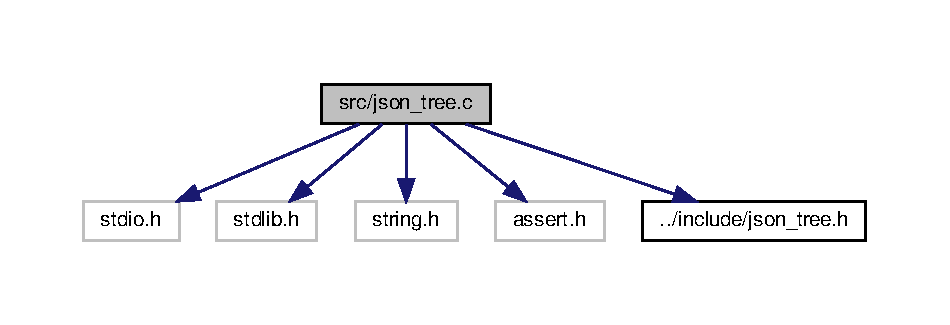
\includegraphics[width=350pt]{json__tree_8c__incl}
\end{center}
\end{figure}
\subsection*{Macros}
\begin{DoxyCompactItemize}
\item 
\mbox{\Hypertarget{json__tree_8c_ad78224efe1d3fb39b67ca74ad9d9eec7}\label{json__tree_8c_ad78224efe1d3fb39b67ca74ad9d9eec7}} 
\#define {\bfseries S\+T\+R\+I\+N\+G\+\_\+\+S\+I\+ZE}~128
\end{DoxyCompactItemize}
\subsection*{Functions}
\begin{DoxyCompactItemize}
\item 
\mbox{\Hypertarget{json__tree_8c_a4a046ddd68dd117c794f1f52df5dad33}\label{json__tree_8c_a4a046ddd68dd117c794f1f52df5dad33}} 
void $\ast$ {\bfseries reallocf} (void $\ast$ptr, size\+\_\+t size)
\item 
\hyperlink{structJsonArray}{Json\+Array} $\ast$ \hyperlink{json__tree_8c_ac6712a1d536004af15b13f93d467de31}{Create\+Json\+Array} ()
\begin{DoxyCompactList}\small\item\em creation en memoire d\textquotesingle{}un \hyperlink{structJsonArray}{Json\+Array} \end{DoxyCompactList}\item 
\mbox{\Hypertarget{json__tree_8c_ae1f0848cee2a75adc68951d7f4e0db94}\label{json__tree_8c_ae1f0848cee2a75adc68951d7f4e0db94}} 
int {\bfseries Insert\+Json\+Array} (\hyperlink{structJsonArray}{Json\+Array} $\ast$\+\_\+array, \hyperlink{structJsonValueContainer}{Json\+Value\+Container} $\ast$\+\_\+value\+Container, const unsigned int \+\_\+position)
\item 
\mbox{\Hypertarget{json__tree_8c_a61372b2f4a3eb734f752159f6265940d}\label{json__tree_8c_a61372b2f4a3eb734f752159f6265940d}} 
int {\bfseries Delete\+Json\+Array} (\hyperlink{structJsonArray}{Json\+Array} $\ast$$\ast$\+\_\+array)
\item 
\mbox{\Hypertarget{json__tree_8c_a30b5080b3f6aba1bbf430aac34d912f7}\label{json__tree_8c_a30b5080b3f6aba1bbf430aac34d912f7}} 
char $\ast$ {\bfseries Print\+Json\+Array} (const \hyperlink{structJsonArray}{Json\+Array} $\ast$\+\_\+array)
\item 
\mbox{\Hypertarget{json__tree_8c_a60f3e947d378f0d1513a6a2495110e0f}\label{json__tree_8c_a60f3e947d378f0d1513a6a2495110e0f}} 
char $\ast$ {\bfseries Print\+Dot\+Json\+Array} (const \hyperlink{structJsonArray}{Json\+Array} $\ast$\+\_\+array)
\item 
\hyperlink{structJsonObject}{Json\+Object} $\ast$ \hyperlink{json__tree_8c_a3808231980cfe4ba4c790a350a294bb7}{Create\+Json\+Object} ()
\begin{DoxyCompactList}\small\item\em construit un \hyperlink{structJsonObject}{Json\+Object} vide \end{DoxyCompactList}\item 
\mbox{\Hypertarget{json__tree_8c_add92f2aba1fffe0af85073527c95fc0e}\label{json__tree_8c_add92f2aba1fffe0af85073527c95fc0e}} 
int {\bfseries Insert\+Json\+Object} (\hyperlink{structJsonObject}{Json\+Object} $\ast$\+\_\+object, \hyperlink{structJsonPair}{Json\+Pair} $\ast$\+\_\+pair)
\item 
\mbox{\Hypertarget{json__tree_8c_af308a2f032f23582b09b7a0238f8f268}\label{json__tree_8c_af308a2f032f23582b09b7a0238f8f268}} 
\hyperlink{structJsonValueContainer}{Json\+Value\+Container} $\ast$ {\bfseries Get\+Json\+Value\+Container} (const \hyperlink{structJsonObject}{Json\+Object} $\ast$\+\_\+object, const char $\ast$\+\_\+string)
\item 
\mbox{\Hypertarget{json__tree_8c_ab9fcb0ea6aba690197eeaa9170d6e279}\label{json__tree_8c_ab9fcb0ea6aba690197eeaa9170d6e279}} 
int {\bfseries Delete\+Json\+Object} (\hyperlink{structJsonObject}{Json\+Object} $\ast$$\ast$\+\_\+object)
\item 
\mbox{\Hypertarget{json__tree_8c_ae153464704693dc8283f34792b4c0a2e}\label{json__tree_8c_ae153464704693dc8283f34792b4c0a2e}} 
char $\ast$ {\bfseries Print\+Json\+Object} (const \hyperlink{structJsonObject}{Json\+Object} $\ast$\+\_\+object)
\item 
\mbox{\Hypertarget{json__tree_8c_a995ed6708039e3e415e5baf8d00ea62e}\label{json__tree_8c_a995ed6708039e3e415e5baf8d00ea62e}} 
char $\ast$ {\bfseries Print\+Dot\+Json\+Object} (const \hyperlink{structJsonObject}{Json\+Object} $\ast$\+\_\+object, int \+\_\+id, int \+\_\+id\+Parent)
\item 
\hyperlink{structJsonValueContainer}{Json\+Value\+Container} $\ast$ \hyperlink{json__tree_8c_a149a190f38e20e9a16c435aaaab14f13}{Create\+Json\+Value\+Container} ()
\begin{DoxyCompactList}\small\item\em construit un \hyperlink{structJsonValueContainer}{Json\+Value\+Container} vide \end{DoxyCompactList}\item 
\mbox{\Hypertarget{json__tree_8c_a918da5f7ca94d6544f77bef2fb75c177}\label{json__tree_8c_a918da5f7ca94d6544f77bef2fb75c177}} 
void {\bfseries Update\+Json\+Value\+Container} (\hyperlink{structJsonValueContainer}{Json\+Value\+Container} $\ast$\+\_\+value\+Container, Value\+Type \+\_\+type, \hyperlink{unionJsonValue}{Json\+Value} \+\_\+value)
\item 
\mbox{\Hypertarget{json__tree_8c_a6d02f560a673f8f70aec2c88d8e32d2d}\label{json__tree_8c_a6d02f560a673f8f70aec2c88d8e32d2d}} 
int {\bfseries Delete\+Json\+Value\+Container} (\hyperlink{structJsonValueContainer}{Json\+Value\+Container} $\ast$$\ast$\+\_\+value\+Container)
\item 
\mbox{\Hypertarget{json__tree_8c_ac93a83ad1ed7f56dd9ecd83e5dfdbdb6}\label{json__tree_8c_ac93a83ad1ed7f56dd9ecd83e5dfdbdb6}} 
char $\ast$ {\bfseries Print\+Json\+Value\+Container} (const \hyperlink{structJsonValueContainer}{Json\+Value\+Container} $\ast$\+\_\+value\+Container)
\item 
\hyperlink{structJsonPair}{Json\+Pair} $\ast$ \hyperlink{json__tree_8c_a7ec4b678b2ea98d4d0f5894460e604b0}{Create\+Json\+Pair} ()
\item 
\mbox{\Hypertarget{json__tree_8c_a028e96028bb843d57b69aecb42b50df1}\label{json__tree_8c_a028e96028bb843d57b69aecb42b50df1}} 
void {\bfseries Update\+Json\+Pair} (\hyperlink{structJsonPair}{Json\+Pair} $\ast$\+\_\+pair, char $\ast$\+\_\+string, \hyperlink{structJsonValueContainer}{Json\+Value\+Container} $\ast$\+\_\+value)
\item 
\mbox{\Hypertarget{json__tree_8c_abcd2910290251bc96cec45cf46d364b7}\label{json__tree_8c_abcd2910290251bc96cec45cf46d364b7}} 
int {\bfseries Delete\+Json\+Pair} (\hyperlink{structJsonPair}{Json\+Pair} $\ast$$\ast$\+\_\+pair)
\item 
\mbox{\Hypertarget{json__tree_8c_aa520ede60813d831e4d92fa2061ed0c4}\label{json__tree_8c_aa520ede60813d831e4d92fa2061ed0c4}} 
char $\ast$ {\bfseries Print\+Json\+Pair} (const \hyperlink{structJsonPair}{Json\+Pair} $\ast$\+\_\+pair)
\end{DoxyCompactItemize}


\subsection{Detailed Description}
implemente la mise en memoire d\textquotesingle{}un arbre json 

\begin{DoxyAuthor}{Author}
NM 
\end{DoxyAuthor}
\begin{DoxyVersion}{Version}
0.\+2 
\end{DoxyVersion}
\begin{DoxyDate}{Date}
20.\+12.\+2018 
\end{DoxyDate}


\subsection{Function Documentation}
\mbox{\Hypertarget{json__tree_8c_ac6712a1d536004af15b13f93d467de31}\label{json__tree_8c_ac6712a1d536004af15b13f93d467de31}} 
\index{json\+\_\+tree.\+c@{json\+\_\+tree.\+c}!Create\+Json\+Array@{Create\+Json\+Array}}
\index{Create\+Json\+Array@{Create\+Json\+Array}!json\+\_\+tree.\+c@{json\+\_\+tree.\+c}}
\subsubsection{\texorpdfstring{Create\+Json\+Array()}{CreateJsonArray()}}
{\footnotesize\ttfamily Create\+Json\+Array (\begin{DoxyParamCaption}{ }\end{DoxyParamCaption})}



creation en memoire d\textquotesingle{}un \hyperlink{structJsonArray}{Json\+Array} 

\begin{DoxyReturn}{Returns}
Json\+Array$\ast$ 
\end{DoxyReturn}
\mbox{\Hypertarget{json__tree_8c_a3808231980cfe4ba4c790a350a294bb7}\label{json__tree_8c_a3808231980cfe4ba4c790a350a294bb7}} 
\index{json\+\_\+tree.\+c@{json\+\_\+tree.\+c}!Create\+Json\+Object@{Create\+Json\+Object}}
\index{Create\+Json\+Object@{Create\+Json\+Object}!json\+\_\+tree.\+c@{json\+\_\+tree.\+c}}
\subsubsection{\texorpdfstring{Create\+Json\+Object()}{CreateJsonObject()}}
{\footnotesize\ttfamily Create\+Json\+Object (\begin{DoxyParamCaption}{ }\end{DoxyParamCaption})}



construit un \hyperlink{structJsonObject}{Json\+Object} vide 

\begin{DoxyReturn}{Returns}
\hyperlink{structJsonObject}{Json\+Object} $\ast$ 
\end{DoxyReturn}
\mbox{\Hypertarget{json__tree_8c_a7ec4b678b2ea98d4d0f5894460e604b0}\label{json__tree_8c_a7ec4b678b2ea98d4d0f5894460e604b0}} 
\index{json\+\_\+tree.\+c@{json\+\_\+tree.\+c}!Create\+Json\+Pair@{Create\+Json\+Pair}}
\index{Create\+Json\+Pair@{Create\+Json\+Pair}!json\+\_\+tree.\+c@{json\+\_\+tree.\+c}}
\subsubsection{\texorpdfstring{Create\+Json\+Pair()}{CreateJsonPair()}}
{\footnotesize\ttfamily Create\+Json\+Pair (\begin{DoxyParamCaption}{ }\end{DoxyParamCaption})}


\begin{DoxyParams}{Parameters}
{\em } & \\
\hline
\end{DoxyParams}
\mbox{\Hypertarget{json__tree_8c_a149a190f38e20e9a16c435aaaab14f13}\label{json__tree_8c_a149a190f38e20e9a16c435aaaab14f13}} 
\index{json\+\_\+tree.\+c@{json\+\_\+tree.\+c}!Create\+Json\+Value\+Container@{Create\+Json\+Value\+Container}}
\index{Create\+Json\+Value\+Container@{Create\+Json\+Value\+Container}!json\+\_\+tree.\+c@{json\+\_\+tree.\+c}}
\subsubsection{\texorpdfstring{Create\+Json\+Value\+Container()}{CreateJsonValueContainer()}}
{\footnotesize\ttfamily Create\+Json\+Value\+Container (\begin{DoxyParamCaption}{ }\end{DoxyParamCaption})}



construit un \hyperlink{structJsonValueContainer}{Json\+Value\+Container} vide 


\begin{DoxyParams}{Parameters}
{\em } & \\
\hline
\end{DoxyParams}

\hypertarget{pile_8c}{}\section{src/pile.c File Reference}
\label{pile_8c}\index{src/pile.\+c@{src/pile.\+c}}


gestion d\textquotesingle{}une pile  


{\ttfamily \#include $<$stdio.\+h$>$}\newline
{\ttfamily \#include $<$stdlib.\+h$>$}\newline
{\ttfamily \#include $<$assert.\+h$>$}\newline
{\ttfamily \#include \char`\"{}../include/pile.\+h\char`\"{}}\newline
Include dependency graph for pile.\+c\+:\nopagebreak
\begin{figure}[H]
\begin{center}
\leavevmode
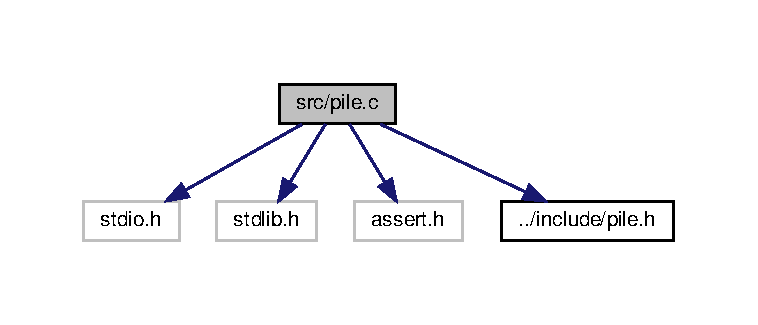
\includegraphics[width=350pt]{pile_8c__incl}
\end{center}
\end{figure}
\subsection*{Macros}
\begin{DoxyCompactItemize}
\item 
\#define \hyperlink{pile_8c_a668c3ac647c6201186c60203494e5ddf}{\+\_\+\+D\+E\+F\+A\+U\+L\+T\+\_\+\+P\+I\+L\+E\+\_\+\+S\+I\+ZE}~15
\end{DoxyCompactItemize}
\subsection*{Functions}
\begin{DoxyCompactItemize}
\item 
\mbox{\Hypertarget{pile_8c_a401766bcab875227f3fe0b4a2c314d9b}\label{pile_8c_a401766bcab875227f3fe0b4a2c314d9b}} 
\hyperlink{structTIntPile}{T\+Int\+Pile} $\ast$ {\bfseries init\+Int\+Pile} ()
\item 
void \hyperlink{pile_8c_a4d8c955ed39c0e02ff16c2583240b4c3}{delete\+Int\+Pile} (\hyperlink{structTIntPile}{T\+Int\+Pile} $\ast$$\ast$\+\_\+pile)
\begin{DoxyCompactList}\small\item\em efface la memoire occupe par la pile \end{DoxyCompactList}\item 
void \hyperlink{pile_8c_a525764cab275369f56d230e3a911cfb6}{print\+Int\+Pile} (\hyperlink{structTIntPile}{T\+Int\+Pile} $\ast$\+\_\+pile)
\begin{DoxyCompactList}\small\item\em affichage du contenu d\textquotesingle{}une pile \end{DoxyCompactList}\item 
void \hyperlink{pile_8c_aca7a8bc8998e15add0598f09a65afa97}{empiler\+Int} (\hyperlink{structTIntPile}{T\+Int\+Pile} $\ast$\+\_\+pile, int \+\_\+val)
\begin{DoxyCompactList}\small\item\em empiler un entier sur la pile, si la zone memoire reservee n\textquotesingle{}est pas suffisante, celle-\/ci est etendue \end{DoxyCompactList}\item 
int \hyperlink{pile_8c_a823ba490199cf04477b74b070e22f3be}{depiler\+Int} (\hyperlink{structTIntPile}{T\+Int\+Pile} $\ast$\+\_\+pile)
\begin{DoxyCompactList}\small\item\em dépiler un entier \end{DoxyCompactList}\item 
int \hyperlink{pile_8c_a8f2c03c053b2b6b9540eeeff20baa086}{sommet\+Int} (\hyperlink{structTIntPile}{T\+Int\+Pile} $\ast$\+\_\+pile)
\begin{DoxyCompactList}\small\item\em renvoie la valeur du sommet (sans depiler) \end{DoxyCompactList}\item 
\hyperlink{structTVoidPile}{T\+Void\+Pile} $\ast$ \hyperlink{pile_8c_a5e8008644ed4ab4223437e2bc12b8f44}{init\+Void\+Pile} ()
\begin{DoxyCompactList}\small\item\em fonction qui initialise une pile de pointeur void $\ast$ \end{DoxyCompactList}\item 
void \hyperlink{pile_8c_a1471f95a65ffd6cc6f3ddeccde2ab327}{delete\+Void\+Pile} (\hyperlink{structTVoidPile}{T\+Void\+Pile} $\ast$$\ast$\+\_\+pile)
\begin{DoxyCompactList}\small\item\em libere la memoire occupee par la pile \end{DoxyCompactList}\item 
void \hyperlink{pile_8c_aa2185907bdfe2791481e174384c41253}{print\+Void\+Pile} (\hyperlink{structTVoidPile}{T\+Void\+Pile} $\ast$\+\_\+pile)
\begin{DoxyCompactList}\small\item\em affichage de la pile (comme on ne connait pas les type des elements empiles, on affiche les adresses de tous les pointeurs empiles) \end{DoxyCompactList}\item 
void \hyperlink{pile_8c_ade2214f96e200aafa5ef341103943de6}{empiler\+Void} (\hyperlink{structTVoidPile}{T\+Void\+Pile} $\ast$\+\_\+pile, void $\ast$\+\_\+val)
\begin{DoxyCompactList}\small\item\em empile un void $\ast$ \end{DoxyCompactList}\item 
void $\ast$ \hyperlink{pile_8c_a6581874a25b111d66cc4b3743ef29b58}{depiler\+Void} (\hyperlink{structTVoidPile}{T\+Void\+Pile} $\ast$\+\_\+pile)
\begin{DoxyCompactList}\small\item\em dépiler un élément de type void $\ast$ \end{DoxyCompactList}\item 
void $\ast$ \hyperlink{pile_8c_affeb266370723f8b2061f34e8650c95e}{sommet\+Void} (\hyperlink{structTVoidPile}{T\+Void\+Pile} $\ast$\+\_\+pile)
\begin{DoxyCompactList}\small\item\em obtenir la valeur du sommet de type void $\ast$ \end{DoxyCompactList}\end{DoxyCompactItemize}


\subsection{Detailed Description}
gestion d\textquotesingle{}une pile 

\begin{DoxyAuthor}{Author}
NM 
\end{DoxyAuthor}
\begin{DoxyVersion}{Version}
0.\+1 
\end{DoxyVersion}
\begin{DoxyDate}{Date}
11/12/2015 
\end{DoxyDate}


\subsection{Macro Definition Documentation}
\mbox{\Hypertarget{pile_8c_a668c3ac647c6201186c60203494e5ddf}\label{pile_8c_a668c3ac647c6201186c60203494e5ddf}} 
\index{pile.\+c@{pile.\+c}!\+\_\+\+D\+E\+F\+A\+U\+L\+T\+\_\+\+P\+I\+L\+E\+\_\+\+S\+I\+ZE@{\+\_\+\+D\+E\+F\+A\+U\+L\+T\+\_\+\+P\+I\+L\+E\+\_\+\+S\+I\+ZE}}
\index{\+\_\+\+D\+E\+F\+A\+U\+L\+T\+\_\+\+P\+I\+L\+E\+\_\+\+S\+I\+ZE@{\+\_\+\+D\+E\+F\+A\+U\+L\+T\+\_\+\+P\+I\+L\+E\+\_\+\+S\+I\+ZE}!pile.\+c@{pile.\+c}}
\subsubsection{\texorpdfstring{\+\_\+\+D\+E\+F\+A\+U\+L\+T\+\_\+\+P\+I\+L\+E\+\_\+\+S\+I\+ZE}{\_DEFAULT\_PILE\_SIZE}}
{\footnotesize\ttfamily \#define \+\_\+\+D\+E\+F\+A\+U\+L\+T\+\_\+\+P\+I\+L\+E\+\_\+\+S\+I\+ZE~15}

constante pour la taille par defaut d\textquotesingle{}une pile (utilise pour la reservation memoire) 

\subsection{Function Documentation}
\mbox{\Hypertarget{pile_8c_a4d8c955ed39c0e02ff16c2583240b4c3}\label{pile_8c_a4d8c955ed39c0e02ff16c2583240b4c3}} 
\index{pile.\+c@{pile.\+c}!delete\+Int\+Pile@{delete\+Int\+Pile}}
\index{delete\+Int\+Pile@{delete\+Int\+Pile}!pile.\+c@{pile.\+c}}
\subsubsection{\texorpdfstring{delete\+Int\+Pile()}{deleteIntPile()}}
{\footnotesize\ttfamily void delete\+Int\+Pile (\begin{DoxyParamCaption}\item[{\hyperlink{structTIntPile}{T\+Int\+Pile} $\ast$$\ast$}]{\+\_\+pile }\end{DoxyParamCaption})}



efface la memoire occupe par la pile 


\begin{DoxyParams}{Parameters}
{\em } & \\
\hline
\end{DoxyParams}
\mbox{\Hypertarget{pile_8c_a1471f95a65ffd6cc6f3ddeccde2ab327}\label{pile_8c_a1471f95a65ffd6cc6f3ddeccde2ab327}} 
\index{pile.\+c@{pile.\+c}!delete\+Void\+Pile@{delete\+Void\+Pile}}
\index{delete\+Void\+Pile@{delete\+Void\+Pile}!pile.\+c@{pile.\+c}}
\subsubsection{\texorpdfstring{delete\+Void\+Pile()}{deleteVoidPile()}}
{\footnotesize\ttfamily void delete\+Void\+Pile (\begin{DoxyParamCaption}\item[{\hyperlink{structTVoidPile}{T\+Void\+Pile} $\ast$$\ast$}]{\+\_\+pile }\end{DoxyParamCaption})}



libere la memoire occupee par la pile 


\begin{DoxyParams}[1]{Parameters}
\mbox{\tt in}  & {\em \+\_\+pile} & \+: adresse du pointeur sur la pile a liberer \\
\hline
\end{DoxyParams}
\begin{DoxyReturn}{Returns}
neant 
\end{DoxyReturn}
\mbox{\Hypertarget{pile_8c_a823ba490199cf04477b74b070e22f3be}\label{pile_8c_a823ba490199cf04477b74b070e22f3be}} 
\index{pile.\+c@{pile.\+c}!depiler\+Int@{depiler\+Int}}
\index{depiler\+Int@{depiler\+Int}!pile.\+c@{pile.\+c}}
\subsubsection{\texorpdfstring{depiler\+Int()}{depilerInt()}}
{\footnotesize\ttfamily int depiler\+Int (\begin{DoxyParamCaption}\item[{\hyperlink{structTIntPile}{T\+Int\+Pile} $\ast$}]{\+\_\+pile }\end{DoxyParamCaption})}



dépiler un entier 


\begin{DoxyParams}[1]{Parameters}
\mbox{\tt in}  & {\em \+\_\+pile} & \+: la pile a depiler \\
\hline
\end{DoxyParams}
\begin{DoxyReturn}{Returns}
l\textquotesingle{}entier en sommet de pile (0 si la pile est vide) 
\end{DoxyReturn}
\mbox{\Hypertarget{pile_8c_a6581874a25b111d66cc4b3743ef29b58}\label{pile_8c_a6581874a25b111d66cc4b3743ef29b58}} 
\index{pile.\+c@{pile.\+c}!depiler\+Void@{depiler\+Void}}
\index{depiler\+Void@{depiler\+Void}!pile.\+c@{pile.\+c}}
\subsubsection{\texorpdfstring{depiler\+Void()}{depilerVoid()}}
{\footnotesize\ttfamily void $\ast$ depiler\+Void (\begin{DoxyParamCaption}\item[{\hyperlink{structTVoidPile}{T\+Void\+Pile} $\ast$}]{\+\_\+pile }\end{DoxyParamCaption})}



dépiler un élément de type void $\ast$ 


\begin{DoxyParams}[1]{Parameters}
\mbox{\tt in}  & {\em \+\_\+pile} & \+: pile a utiliser \\
\hline
\end{DoxyParams}
\begin{DoxyReturn}{Returns}
pointeur sur void (0 si la pile est vide) 
\end{DoxyReturn}
\mbox{\Hypertarget{pile_8c_aca7a8bc8998e15add0598f09a65afa97}\label{pile_8c_aca7a8bc8998e15add0598f09a65afa97}} 
\index{pile.\+c@{pile.\+c}!empiler\+Int@{empiler\+Int}}
\index{empiler\+Int@{empiler\+Int}!pile.\+c@{pile.\+c}}
\subsubsection{\texorpdfstring{empiler\+Int()}{empilerInt()}}
{\footnotesize\ttfamily void empiler\+Int (\begin{DoxyParamCaption}\item[{\hyperlink{structTIntPile}{T\+Int\+Pile} $\ast$}]{\+\_\+pile,  }\item[{int}]{\+\_\+val }\end{DoxyParamCaption})}



empiler un entier sur la pile, si la zone memoire reservee n\textquotesingle{}est pas suffisante, celle-\/ci est etendue 


\begin{DoxyParams}{Parameters}
{\em } & \\
\hline
\end{DoxyParams}
\mbox{\Hypertarget{pile_8c_ade2214f96e200aafa5ef341103943de6}\label{pile_8c_ade2214f96e200aafa5ef341103943de6}} 
\index{pile.\+c@{pile.\+c}!empiler\+Void@{empiler\+Void}}
\index{empiler\+Void@{empiler\+Void}!pile.\+c@{pile.\+c}}
\subsubsection{\texorpdfstring{empiler\+Void()}{empilerVoid()}}
{\footnotesize\ttfamily void empiler\+Void (\begin{DoxyParamCaption}\item[{\hyperlink{structTVoidPile}{T\+Void\+Pile} $\ast$}]{\+\_\+pile,  }\item[{void $\ast$}]{\+\_\+val }\end{DoxyParamCaption})}



empile un void $\ast$ 


\begin{DoxyParams}{Parameters}
{\em } & \\
\hline
\end{DoxyParams}
\mbox{\Hypertarget{pile_8c_a5e8008644ed4ab4223437e2bc12b8f44}\label{pile_8c_a5e8008644ed4ab4223437e2bc12b8f44}} 
\index{pile.\+c@{pile.\+c}!init\+Void\+Pile@{init\+Void\+Pile}}
\index{init\+Void\+Pile@{init\+Void\+Pile}!pile.\+c@{pile.\+c}}
\subsubsection{\texorpdfstring{init\+Void\+Pile()}{initVoidPile()}}
{\footnotesize\ttfamily \hyperlink{structTVoidPile}{T\+Void\+Pile} $\ast$ init\+Void\+Pile (\begin{DoxyParamCaption}{ }\end{DoxyParamCaption})}



fonction qui initialise une pile de pointeur void $\ast$ 

pile de void $\ast$ -\/-\/-\/-\/-\/-\/-\/-\/-\/-\/-\/-\/-\/-\/-\/-\/-\/-\/-\/-\/-\/-\/-\/-\/-\/-\/-\/-\/-\/-\/-\/-\/-\/-\/-\/-\/-\/-\/-\/-\/-\/-\/-\/-\/-\/------

\begin{DoxyReturn}{Returns}
pointeur sur une pile \hyperlink{structTVoidPile}{T\+Void\+Pile} 
\end{DoxyReturn}
\mbox{\Hypertarget{pile_8c_a525764cab275369f56d230e3a911cfb6}\label{pile_8c_a525764cab275369f56d230e3a911cfb6}} 
\index{pile.\+c@{pile.\+c}!print\+Int\+Pile@{print\+Int\+Pile}}
\index{print\+Int\+Pile@{print\+Int\+Pile}!pile.\+c@{pile.\+c}}
\subsubsection{\texorpdfstring{print\+Int\+Pile()}{printIntPile()}}
{\footnotesize\ttfamily void print\+Int\+Pile (\begin{DoxyParamCaption}\item[{\hyperlink{structTIntPile}{T\+Int\+Pile} $\ast$}]{\+\_\+pile }\end{DoxyParamCaption})}



affichage du contenu d\textquotesingle{}une pile 


\begin{DoxyParams}[1]{Parameters}
\mbox{\tt in}  & {\em \+\_\+pile} & \+: la pile a afficher \\
\hline
\end{DoxyParams}
\begin{DoxyReturn}{Returns}
neant 
\end{DoxyReturn}
\mbox{\Hypertarget{pile_8c_aa2185907bdfe2791481e174384c41253}\label{pile_8c_aa2185907bdfe2791481e174384c41253}} 
\index{pile.\+c@{pile.\+c}!print\+Void\+Pile@{print\+Void\+Pile}}
\index{print\+Void\+Pile@{print\+Void\+Pile}!pile.\+c@{pile.\+c}}
\subsubsection{\texorpdfstring{print\+Void\+Pile()}{printVoidPile()}}
{\footnotesize\ttfamily void print\+Void\+Pile (\begin{DoxyParamCaption}\item[{\hyperlink{structTVoidPile}{T\+Void\+Pile} $\ast$}]{\+\_\+pile }\end{DoxyParamCaption})}



affichage de la pile (comme on ne connait pas les type des elements empiles, on affiche les adresses de tous les pointeurs empiles) 


\begin{DoxyParams}[1]{Parameters}
\mbox{\tt in}  & {\em \+\_\+pile} & \+: pile a afficher \\
\hline
\end{DoxyParams}
\begin{DoxyReturn}{Returns}
neant 
\end{DoxyReturn}
\mbox{\Hypertarget{pile_8c_a8f2c03c053b2b6b9540eeeff20baa086}\label{pile_8c_a8f2c03c053b2b6b9540eeeff20baa086}} 
\index{pile.\+c@{pile.\+c}!sommet\+Int@{sommet\+Int}}
\index{sommet\+Int@{sommet\+Int}!pile.\+c@{pile.\+c}}
\subsubsection{\texorpdfstring{sommet\+Int()}{sommetInt()}}
{\footnotesize\ttfamily int sommet\+Int (\begin{DoxyParamCaption}\item[{\hyperlink{structTIntPile}{T\+Int\+Pile} $\ast$}]{\+\_\+pile }\end{DoxyParamCaption})}



renvoie la valeur du sommet (sans depiler) 


\begin{DoxyParams}[1]{Parameters}
\mbox{\tt in}  & {\em \+\_\+pile} & \+: la pile a utiliser \\
\hline
\end{DoxyParams}
\begin{DoxyReturn}{Returns}
l\textquotesingle{}entier en sommet de pile (0 si la pile est vide) 
\end{DoxyReturn}
\mbox{\Hypertarget{pile_8c_affeb266370723f8b2061f34e8650c95e}\label{pile_8c_affeb266370723f8b2061f34e8650c95e}} 
\index{pile.\+c@{pile.\+c}!sommet\+Void@{sommet\+Void}}
\index{sommet\+Void@{sommet\+Void}!pile.\+c@{pile.\+c}}
\subsubsection{\texorpdfstring{sommet\+Void()}{sommetVoid()}}
{\footnotesize\ttfamily void $\ast$ sommet\+Void (\begin{DoxyParamCaption}\item[{\hyperlink{structTVoidPile}{T\+Void\+Pile} $\ast$}]{\+\_\+pile }\end{DoxyParamCaption})}



obtenir la valeur du sommet de type void $\ast$ 


\begin{DoxyParams}[1]{Parameters}
\mbox{\tt in}  & {\em \+\_\+pile} & \+: pile a utiliser pour lire le sommet \\
\hline
\end{DoxyParams}
\begin{DoxyReturn}{Returns}
la valeur void $\ast$ du sommet (0 si la pile est vide) 
\end{DoxyReturn}

\hypertarget{tp2__lex_8c}{}\section{src/tp2\+\_\+lex.c File Reference}
\label{tp2__lex_8c}\index{src/tp2\+\_\+lex.\+c@{src/tp2\+\_\+lex.\+c}}


analyseur lexical pour le langage J\+S\+ON  


{\ttfamily \#include $<$stdio.\+h$>$}\newline
{\ttfamily \#include $<$string.\+h$>$}\newline
{\ttfamily \#include $<$ctype.\+h$>$}\newline
{\ttfamily \#include $<$stdlib.\+h$>$}\newline
{\ttfamily \#include $<$assert.\+h$>$}\newline
{\ttfamily \#include $<$regex.\+h$>$}\newline
{\ttfamily \#include \char`\"{}../include/tp2\+\_\+lex.\+h\char`\"{}}\newline
Include dependency graph for tp2\+\_\+lex.\+c\+:\nopagebreak
\begin{figure}[H]
\begin{center}
\leavevmode
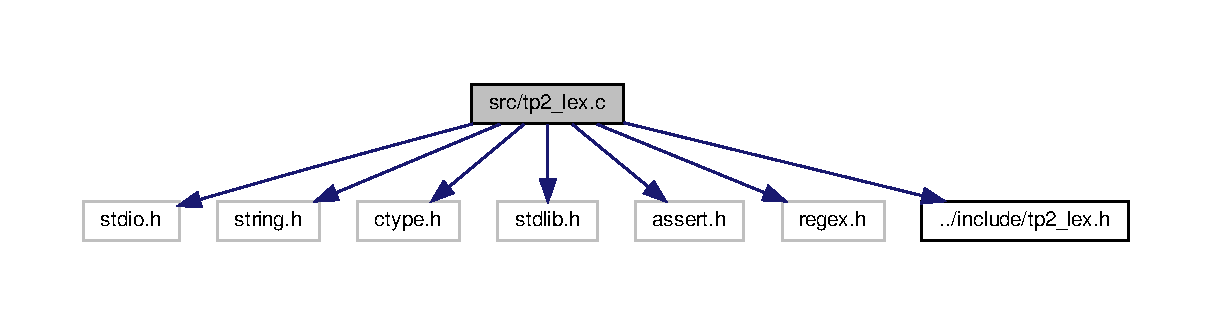
\includegraphics[width=350pt]{tp2__lex_8c__incl}
\end{center}
\end{figure}
\subsection*{Functions}
\begin{DoxyCompactItemize}
\item 
int \hyperlink{tp2__lex_8c_a9869519009e3b965c6401e67261f6c43}{is\+Sep} (const char \+\_\+symb)
\begin{DoxyCompactList}\small\item\em fonction qui teste si un symbole fait partie des separateurs \end{DoxyCompactList}\item 
\hyperlink{structTLex}{T\+Lex} $\ast$ \hyperlink{tp2__lex_8c_ac829e0ab2aa3b0d2e165edefa6be8009}{init\+Lex\+Data} (char $\ast$\+\_\+data)
\begin{DoxyCompactList}\small\item\em fonction qui reserve la memoire et initialise les donnees pour l\textquotesingle{}analyseur lexical \end{DoxyCompactList}\item 
void \hyperlink{tp2__lex_8c_a66ac3a0b39b824a8e72654633945a95f}{delete\+Lex\+Data} (\hyperlink{structTLex}{T\+Lex} $\ast$$\ast$\+\_\+lex\+Data)
\begin{DoxyCompactList}\small\item\em fonction qui supprime de la memoire les donnees pour l\textquotesingle{}analyseur lexical \end{DoxyCompactList}\item 
void \hyperlink{tp2__lex_8c_a5cad73df0d00e5735e16356504a923b1}{print\+Lex\+Data} (\hyperlink{structTLex}{T\+Lex} $\ast$\+\_\+lex\+Data)
\begin{DoxyCompactList}\small\item\em fonction qui affiche les donnees pour l\textquotesingle{}analyseur lexical \end{DoxyCompactList}\item 
int \hyperlink{tp2__lex_8c_afed09d4c5ae5433e332256c311411bb6}{change\+Table\+Symbole\+Size} (\hyperlink{structTLex}{T\+Lex} $\ast$\+\_\+lex\+Data)
\begin{DoxyCompactList}\small\item\em Fonction qui incrémente le nombre de symbole de la table des symbole et augmente sa taille. \end{DoxyCompactList}\item 
void \hyperlink{tp2__lex_8c_a769d490ddf9b2cae334051946a61573b}{add\+Int\+Symbol\+To\+Lex\+Data} (\hyperlink{structTLex}{T\+Lex} $\ast$\+\_\+lex\+Data, const int \+\_\+val)
\begin{DoxyCompactList}\small\item\em fonction qui ajoute un symbole entier a la table des symboles \end{DoxyCompactList}\item 
void \hyperlink{tp2__lex_8c_a42504307caaa42184de9dd79b180b946}{add\+Real\+Symbol\+To\+Lex\+Data} (\hyperlink{structTLex}{T\+Lex} $\ast$\+\_\+lex\+Data, const float \+\_\+val)
\begin{DoxyCompactList}\small\item\em fonction qui ajoute un symbole reel a la table des symboles \end{DoxyCompactList}\item 
void \hyperlink{tp2__lex_8c_acc16ce9abf0d176fbe754943171f5c4e}{add\+String\+Symbol\+To\+Lex\+Data} (\hyperlink{structTLex}{T\+Lex} $\ast$\+\_\+lex\+Data, char $\ast$\+\_\+val)
\begin{DoxyCompactList}\small\item\em fonction qui ajoute une chaine de caracteres a la table des symboles \end{DoxyCompactList}\item 
\mbox{\Hypertarget{tp2__lex_8c_a4f39d3deacca77d7b4cf543101da84a6}\label{tp2__lex_8c_a4f39d3deacca77d7b4cf543101da84a6}} 
int {\bfseries lex} (\hyperlink{structTLex}{T\+Lex} $\ast$\+\_\+lex\+Data)
\end{DoxyCompactItemize}
\subsection*{Variables}
\begin{DoxyCompactItemize}
\item 
\mbox{\Hypertarget{tp2__lex_8c_a55d5c377110e89859a38a0498cc294ef}\label{tp2__lex_8c_a55d5c377110e89859a38a0498cc294ef}} 
char $\ast$ {\bfseries separators} = \char`\"{}\{\}\mbox{[}$\,$\mbox{]},;\textbackslash{}n \textbackslash{}t\char`\"{}
\end{DoxyCompactItemize}


\subsection{Detailed Description}
analyseur lexical pour le langage J\+S\+ON 

\begin{DoxyAuthor}{Author}
NM 
\end{DoxyAuthor}
\begin{DoxyVersion}{Version}
0.\+1 
\end{DoxyVersion}
\begin{DoxyDate}{Date}
25/11/2015 
\end{DoxyDate}


\subsection{Function Documentation}
\mbox{\Hypertarget{tp2__lex_8c_a769d490ddf9b2cae334051946a61573b}\label{tp2__lex_8c_a769d490ddf9b2cae334051946a61573b}} 
\index{tp2\+\_\+lex.\+c@{tp2\+\_\+lex.\+c}!add\+Int\+Symbol\+To\+Lex\+Data@{add\+Int\+Symbol\+To\+Lex\+Data}}
\index{add\+Int\+Symbol\+To\+Lex\+Data@{add\+Int\+Symbol\+To\+Lex\+Data}!tp2\+\_\+lex.\+c@{tp2\+\_\+lex.\+c}}
\subsubsection{\texorpdfstring{add\+Int\+Symbol\+To\+Lex\+Data()}{addIntSymbolToLexData()}}
{\footnotesize\ttfamily void add\+Int\+Symbol\+To\+Lex\+Data (\begin{DoxyParamCaption}\item[{\hyperlink{structTLex}{T\+Lex} $\ast$}]{\+\_\+lex\+Data,  }\item[{const int}]{\+\_\+val }\end{DoxyParamCaption})}



fonction qui ajoute un symbole entier a la table des symboles 


\begin{DoxyParams}[1]{Parameters}
\mbox{\tt in,out}  & {\em \+\_\+lex\+Data} & donnees de l\textquotesingle{}analyseur lexical \\
\hline
\mbox{\tt in}  & {\em \+\_\+val} & valeur entiere e ajouter \\
\hline
\end{DoxyParams}
\begin{DoxyReturn}{Returns}
neant 
\end{DoxyReturn}
\mbox{\Hypertarget{tp2__lex_8c_a42504307caaa42184de9dd79b180b946}\label{tp2__lex_8c_a42504307caaa42184de9dd79b180b946}} 
\index{tp2\+\_\+lex.\+c@{tp2\+\_\+lex.\+c}!add\+Real\+Symbol\+To\+Lex\+Data@{add\+Real\+Symbol\+To\+Lex\+Data}}
\index{add\+Real\+Symbol\+To\+Lex\+Data@{add\+Real\+Symbol\+To\+Lex\+Data}!tp2\+\_\+lex.\+c@{tp2\+\_\+lex.\+c}}
\subsubsection{\texorpdfstring{add\+Real\+Symbol\+To\+Lex\+Data()}{addRealSymbolToLexData()}}
{\footnotesize\ttfamily void add\+Real\+Symbol\+To\+Lex\+Data (\begin{DoxyParamCaption}\item[{\hyperlink{structTLex}{T\+Lex} $\ast$}]{\+\_\+lex\+Data,  }\item[{const float}]{\+\_\+val }\end{DoxyParamCaption})}



fonction qui ajoute un symbole reel a la table des symboles 


\begin{DoxyParams}[1]{Parameters}
\mbox{\tt in,out}  & {\em \+\_\+lex\+Data} & donnees de l\textquotesingle{}analyseur lexical \\
\hline
\mbox{\tt in}  & {\em \+\_\+val} & valeur reelle a ajouter \\
\hline
\end{DoxyParams}
\mbox{\Hypertarget{tp2__lex_8c_acc16ce9abf0d176fbe754943171f5c4e}\label{tp2__lex_8c_acc16ce9abf0d176fbe754943171f5c4e}} 
\index{tp2\+\_\+lex.\+c@{tp2\+\_\+lex.\+c}!add\+String\+Symbol\+To\+Lex\+Data@{add\+String\+Symbol\+To\+Lex\+Data}}
\index{add\+String\+Symbol\+To\+Lex\+Data@{add\+String\+Symbol\+To\+Lex\+Data}!tp2\+\_\+lex.\+c@{tp2\+\_\+lex.\+c}}
\subsubsection{\texorpdfstring{add\+String\+Symbol\+To\+Lex\+Data()}{addStringSymbolToLexData()}}
{\footnotesize\ttfamily void add\+String\+Symbol\+To\+Lex\+Data (\begin{DoxyParamCaption}\item[{\hyperlink{structTLex}{T\+Lex} $\ast$}]{\+\_\+lex\+Data,  }\item[{char $\ast$}]{\+\_\+val }\end{DoxyParamCaption})}



fonction qui ajoute une chaine de caracteres a la table des symboles 


\begin{DoxyParams}[1]{Parameters}
\mbox{\tt in,out}  & {\em \+\_\+lex\+Data} & donnees de l\textquotesingle{}analyseur lexical \\
\hline
\mbox{\tt in}  & {\em \+\_\+val} & chaine a ajouter \\
\hline
\end{DoxyParams}
\mbox{\Hypertarget{tp2__lex_8c_afed09d4c5ae5433e332256c311411bb6}\label{tp2__lex_8c_afed09d4c5ae5433e332256c311411bb6}} 
\index{tp2\+\_\+lex.\+c@{tp2\+\_\+lex.\+c}!change\+Table\+Symbole\+Size@{change\+Table\+Symbole\+Size}}
\index{change\+Table\+Symbole\+Size@{change\+Table\+Symbole\+Size}!tp2\+\_\+lex.\+c@{tp2\+\_\+lex.\+c}}
\subsubsection{\texorpdfstring{change\+Table\+Symbole\+Size()}{changeTableSymboleSize()}}
{\footnotesize\ttfamily int change\+Table\+Symbole\+Size (\begin{DoxyParamCaption}\item[{\hyperlink{structTLex}{T\+Lex} $\ast$}]{\+\_\+lex\+Data }\end{DoxyParamCaption})}



Fonction qui incrémente le nombre de symbole de la table des symbole et augmente sa taille. 


\begin{DoxyParams}[1]{Parameters}
\mbox{\tt in,out}  & {\em \+\_\+lex\+Data} & donnees de l\textquotesingle{}analyseur lexical \\
\hline
\end{DoxyParams}
\begin{DoxyReturn}{Returns}
reallocation reussie 
\end{DoxyReturn}
\mbox{\Hypertarget{tp2__lex_8c_a66ac3a0b39b824a8e72654633945a95f}\label{tp2__lex_8c_a66ac3a0b39b824a8e72654633945a95f}} 
\index{tp2\+\_\+lex.\+c@{tp2\+\_\+lex.\+c}!delete\+Lex\+Data@{delete\+Lex\+Data}}
\index{delete\+Lex\+Data@{delete\+Lex\+Data}!tp2\+\_\+lex.\+c@{tp2\+\_\+lex.\+c}}
\subsubsection{\texorpdfstring{delete\+Lex\+Data()}{deleteLexData()}}
{\footnotesize\ttfamily void delete\+Lex\+Data (\begin{DoxyParamCaption}\item[{\hyperlink{structTLex}{T\+Lex} $\ast$$\ast$}]{\+\_\+lex\+Data }\end{DoxyParamCaption})}



fonction qui supprime de la memoire les donnees pour l\textquotesingle{}analyseur lexical 


\begin{DoxyParams}[1]{Parameters}
\mbox{\tt in,out}  & {\em \+\_\+lex\+Data} & donnees de l\textquotesingle{}analyseur lexical \\
\hline
\end{DoxyParams}
\begin{DoxyReturn}{Returns}
neant 
\end{DoxyReturn}
\mbox{\Hypertarget{tp2__lex_8c_ac829e0ab2aa3b0d2e165edefa6be8009}\label{tp2__lex_8c_ac829e0ab2aa3b0d2e165edefa6be8009}} 
\index{tp2\+\_\+lex.\+c@{tp2\+\_\+lex.\+c}!init\+Lex\+Data@{init\+Lex\+Data}}
\index{init\+Lex\+Data@{init\+Lex\+Data}!tp2\+\_\+lex.\+c@{tp2\+\_\+lex.\+c}}
\subsubsection{\texorpdfstring{init\+Lex\+Data()}{initLexData()}}
{\footnotesize\ttfamily \hyperlink{structTLex}{T\+Lex} $\ast$ init\+Lex\+Data (\begin{DoxyParamCaption}\item[{char $\ast$}]{\+\_\+data }\end{DoxyParamCaption})}



fonction qui reserve la memoire et initialise les donnees pour l\textquotesingle{}analyseur lexical 


\begin{DoxyParams}[1]{Parameters}
\mbox{\tt in}  & {\em \+\_\+data} & chaine a analyser \\
\hline
\end{DoxyParams}
\begin{DoxyReturn}{Returns}
pointeur sur la structure de donnees creee 
\end{DoxyReturn}
\mbox{\Hypertarget{tp2__lex_8c_a9869519009e3b965c6401e67261f6c43}\label{tp2__lex_8c_a9869519009e3b965c6401e67261f6c43}} 
\index{tp2\+\_\+lex.\+c@{tp2\+\_\+lex.\+c}!is\+Sep@{is\+Sep}}
\index{is\+Sep@{is\+Sep}!tp2\+\_\+lex.\+c@{tp2\+\_\+lex.\+c}}
\subsubsection{\texorpdfstring{is\+Sep()}{isSep()}}
{\footnotesize\ttfamily int is\+Sep (\begin{DoxyParamCaption}\item[{const char}]{\+\_\+symb }\end{DoxyParamCaption})}



fonction qui teste si un symbole fait partie des separateurs 


\begin{DoxyParams}[1]{Parameters}
\mbox{\tt in}  & {\em \+\_\+symb} & symbole a analyser \\
\hline
\end{DoxyParams}
\begin{DoxyReturn}{Returns}
1 (vrai) si \+\_\+symb est un separateur, 0 (faux) sinon 
\end{DoxyReturn}
\mbox{\Hypertarget{tp2__lex_8c_a5cad73df0d00e5735e16356504a923b1}\label{tp2__lex_8c_a5cad73df0d00e5735e16356504a923b1}} 
\index{tp2\+\_\+lex.\+c@{tp2\+\_\+lex.\+c}!print\+Lex\+Data@{print\+Lex\+Data}}
\index{print\+Lex\+Data@{print\+Lex\+Data}!tp2\+\_\+lex.\+c@{tp2\+\_\+lex.\+c}}
\subsubsection{\texorpdfstring{print\+Lex\+Data()}{printLexData()}}
{\footnotesize\ttfamily void print\+Lex\+Data (\begin{DoxyParamCaption}\item[{\hyperlink{structTLex}{T\+Lex} $\ast$}]{\+\_\+lex\+Data }\end{DoxyParamCaption})}



fonction qui affiche les donnees pour l\textquotesingle{}analyseur lexical 


\begin{DoxyParams}[1]{Parameters}
\mbox{\tt in}  & {\em \+\_\+lex\+Data} & données de l\textquotesingle{}analyseur lexical \\
\hline
\end{DoxyParams}
\begin{DoxyReturn}{Returns}
neant 
\end{DoxyReturn}

%--- End generated contents ---

% Index
\backmatter
\newpage
\phantomsection
\clearemptydoublepage
\addcontentsline{toc}{chapter}{Index}
\printindex

\end{document}
